\documentclass[12pt,a4paper]{article}

% ============================================
% PAQUETES ESENCIALES
% ============================================
\usepackage[utf8]{inputenc}        
\usepackage[T1]{fontenc}             
\usepackage[spanish,es-tabla]{babel}  

\usepackage{times} 
\usepackage{geometry}
\usepackage{setspace}
\usepackage{graphicx}
\usepackage{titlesec}
\usepackage{fancyhdr}
\usepackage{enumitem}
\usepackage{hyperref}
\usepackage{tabularx}
\usepackage{booktabs}
\usepackage{longtable}
\usepackage{multirow}
\usepackage{pdflscape}
\usepackage{fmtcount}
\usepackage{comment}
\usepackage{float}
\usepackage{caption}
\usepackage{siunitx}
\usepackage{ragged2e}
\usepackage{array}
\usepackage[table]{xcolor}
\usepackage{colortbl} 

% ============================================
% CONFIGURACIÓN DE URLS Y MÁRGENES DE HOJA
% ============================================
\usepackage{url}
\Urlmuskip=0mu plus 1mu 
\makeatletter
\g@addto@macro{\UrlBreaks}{\do\/\do\-\do\.\do\=\do\_\do\?\do\&\do\%}
\makeatother

\geometry{
	a4paper,
	top=2.5cm,
	bottom=2.5cm,
	left=3cm,
	right=2cm
}
\setstretch{1.5}

% ============================================
% PAQUETE TOCLOFT Y CONFIGURACIÓN DE ÍNDICES (APA 7)
% ============================================
\usepackage{tocloft}
% Corrección de colisión horizontal del número romano VII
\setlength{\cftsecnumwidth}{3.2em} 

% Formateo para incluir la palabra "Tabla X" en la lista de tablas
\renewcommand{\cfttabpresnum}{\textbf{Tabla }} 
\setlength{\cfttabnumwidth}{4.5em}             
\renewcommand{\cfttabaftersnumb}{\hspace{0.1em}} 

% Formateo para incluir la palabra "Figura X" en la lista de figuras
\renewcommand{\cftfigpresnum}{\textbf{Figura }} 
\setlength{\cftfignumwidth}{4.8em}             
\renewcommand{\cftfigaftersnumb}{\hspace{0.1em}} 

% ============================================
% CONFIGURACIÓN DE HIPERVÍNCULOS
% ============================================
\hypersetup{
	colorlinks=true,
	linkcolor=black,
	citecolor=black,
	urlcolor=blue,
	pdfencoding=auto
}

% ============================================
% CONFIGURACIÓN DE TÍTULOS
% ============================================
\titleformat{\section}{\normalfont\fontsize{12}{15}\bfseries\uppercase}{\thesection}{1em}{}
\titleformat{\subsection}{\normalfont\fontsize{12}{15}\bfseries}{\thesubsection}{1em}{}
\titleformat{\subsubsection}{\normalfont\fontsize{12}{15}\bfseries}{\thesubsubsection}{1em}{}

% ============================================
% ENCABEZADOS Y PIES DE PÁGINA
% ============================================
\pagestyle{fancy}
\fancyhf{}
\fancyfoot[C]{\thepage}
\renewcommand{\headrulewidth}{0pt}

% ============================================
% CONFIGURACIÓN DE TABLAS SEGÚN APA 7
% ============================================
\captionsetup[table]{
	format=plain,
	labelformat=simple,
	labelsep=newline,
	labelfont=bf,
	textfont=it,
	justification=raggedright,
	singlelinecheck=false,
	position=top
}

% ============================================
% INFORMACIÓN INSTITUCIONAL DEL DOCUMENTO
% ============================================
\newcommand{\universidadLinea}{UNIVERSIDAD NACIONAL}
\newcommand{\universidadLineaDos}{SANTIAGO ANTÚNEZ DE MAYOLO}
\newcommand{\facultad}{FACULTAD DE CIENCIAS}
\newcommand{\escuela}{ESCUELA PROFESIONAL DE INGENIERÍA DE SISTEMAS E INFORMÁTICA}
\newcommand{\tituloTesis}{PROTOTIPO DE SMART PARKING SYSTEM APLICANDO TECNOLOGÍAS EMERGENTES DE INTERNET OF THINGS, ARTIFICIAL INTELLIGENCE Y CLOUD COMPUTING PARA UNA SMART MOBILITY DE SMART CITY EN HUARAZ - ÁNCASH, 2025}
\newcommand{\autor}{EDWIN YONER FLORES RUPAY}
\newcommand{\asesor}{FRANZ MARTÍN VILLANUEVA COCHACHIN} 
\newcommand{\ciudad}{Huaraz}
\newcommand{\anio}{2026}

% ============================================
% CUERPO PRINCIPAL DEL DOCUMENTO
% ============================================
\begin{document}
	
	\pagenumbering{gobble}
	
	% ============================================
	% CARÁTULA O PORTADA
	% ============================================
	\begin{titlepage}
		\centering
		\setstretch{1.2}
		{\large\bfseries \universidadLinea \par}
		{\large\bfseries \universidadLineaDos \par}
		\vspace{0.5cm}
		{\large\bfseries \facultad \par}
		\vspace{0.5cm}
		{\large\bfseries \escuela \par}
		\vspace{0.8cm}
		
		\includegraphics[width=0.25\textwidth]{logo_unasam.png}
		\vspace{0.8cm}
		
		{\Large\bfseries PROYECTO DE TESIS \par}
		\vspace{0.75cm}
		
		{\normalsize\bfseries \tituloTesis \par}
		\vfill
		
		{\large PRESENTADO POR: \par}
		\vspace{0.3cm}
		{\large Bachiller: \autor \par}
		\vspace{1cm}
		
		{\large ASESOR: \par}
		\vspace{0.3cm}
		{\large Maestro: \asesor \par}
		\vfill
		
		{\large HUARAZ - PERÚ \par}
		{\large \anio \par}
	\end{titlepage}
	
	% ============================================
	% SECCIÓN DE ÍNDICES PRELIMINARES
	% ============================================
	\clearpage
	\pagenumbering{Roman}
	\setcounter{page}{1}
	
	% 1. Índice General (Contenido)
	\renewcommand{\contentsname}{CONTENIDO}
	\tableofcontents
	\clearpage
	
	% 2. Índice de Tablas (Lista de tablas con prefijo automático)
	\renewcommand{\listtablename}{ÍNDICE DE TABLAS}
	\phantomsection % <-- CREA EL ANCLA CORRECTA DE HIPERVÍNCULO AQUÍ
	\addcontentsline{toc}{section}{\listtablename}
	\listoftables
	\clearpage
	
	% 3. Índice de Figuras (Lista de figuras con prefijo automático)
	\renewcommand{\listfigurename}{ÍNDICE DE FIGURAS}
	\phantomsection % <-- CREA EL ANCLA CORRECTA DE HIPERVÍNCULO AQUÍ
	\addcontentsline{toc}{section}{\listfigurename}
	\listoffigures
	\clearpage
	
% ============================================
% PRIMERA PARTE: DATOS GENERALES
% ============================================
\phantomsection % <-- CREA EL ANCLA CORRECTA PARA ESTE TÍTULO SIN NÚMERO
\section*{PRIMERA PARTE: DATOS GENERALES}
\addcontentsline{toc}{section}{PRIMERA PARTE: DATOS GENERALES}

\subsection*{1. TÍTULO}
\addcontentsline{toc}{subsection}{1. Título}
\tituloTesis

\subsection*{2. AUTOR}
\addcontentsline{toc}{subsection}{2. Autor}
\begin{itemize}[leftmargin=*]
    \item \textbf{Apellidos y nombres:} Flores Rupay Edwin Yoner
\end{itemize}

\subsection*{3. ASESOR}
\addcontentsline{toc}{subsection}{3. Asesor}
\begin{itemize}[leftmargin=*]
    \item \textbf{Apellidos y nombres:} Villanueva Cochachin Franz Martín
    \item \textbf{Grado académico:} Maestro en ciencias e ingeniería con mención en auditoría y seguridad informática
    \item \textbf{Título profesional:} Ingeniero Electrónico
    \item \textbf{Dirección laboral:} Universidad Nacional Santiago Antúnez De Mayolo\\
    Av. Universitaria S/N – Barrio Shancayan - Distrito de Independencia
\end{itemize}

\begin{comment}
\subsection*{4. LÍNEA Y SUBLÍNEA DE INVESTIGACIÓN}
\addcontentsline{toc}{subsection}{4. Línea y sublínea de investigación}
\begin{itemize}[leftmargin=*]
    \item \textbf{Línea de investigación:} Energía Renovable E Innovación Tecnológica
    \item \textbf{Sublínea de investigación:} Ciencia De Datos E Ingeniería Para La Inteligencia Artificial
\end{itemize}
\end{comment}

\subsection*{4. LÍNEA Y SUBLÍNEA DE INVESTIGACIÓN}
\addcontentsline{toc}{subsection}{4. Línea y sublínea de investigación}
\begin{itemize}[leftmargin=*]
	\item \textbf{Área de investigación:} Ingeniería y Tecnología
	\item \textbf{Línea de investigación:} Energía Renovable e Innovación Tecnológica
	\item \textbf{Sublíneas de investigación:} 
	\begin{itemize}
		\item Ciencia de datos e ingeniería para la inteligencia artificial
		\item Sistema de información e ingeniería de software
		\item Seguridad, negocios electrónicos, Cloud computing y gestión de bases de datos
		\item Redes de telecomunicaciones, sistemas electrónicos, digitales y de control
	\end{itemize}
\end{itemize}

\subsection*{5. TIPO DE INVESTIGACIÓN}
\addcontentsline{toc}{subsection}{5. Tipo de investigación}

\subsubsection*{5.1. De acuerdo a la orientación}
\addcontentsline{toc}{subsubsection}{5.1. De acuerdo a la orientación}
\textbf{Aplicada:} La investigación está orientada a desarrollar un prototipo destinado a contribuir a la solución de problemas relacionados con la gestión de parqueos en la ciudad de Huaraz, contribuyendo al desarrollo de ciudades inteligentes en la región.

\subsubsection*{5.2. De acuerdo a la técnica de contrastación}
\addcontentsline{toc}{subsubsection}{5.2. De acuerdo a la técnica de contrastación} 
\textbf{Explicativa:} Se utilizará experimentación mediante el desarrollo e implementación de un prototipo que integra tecnologías Internet of Things, Artificial Intelligence y Cloud Computing. Los datos serán obtenidos por observación de fenómenos condicionados por el investigador, evaluando variables de rendimiento, eficiencia y usabilidad en escenarios controlados de gestión de parqueos.

\subsection*{6. RÉGIMEN DE INVESTIGACIÓN}
\addcontentsline{toc}{subsection}{6. Régimen de investigación}

\textbf{Orientada:} El tema de investigación se encuentra alineado con las líneas de investigación de la Facultad de Ciencias, específicamente dentro del área de \textbf{Ingeniería y Tecnología}, línea de investigación \textbf{Energía Renovable e Innovación Tecnológica}, aprobadas según el documento "Líneas de Investigación de la UNASAM" del Vicerrectorado de Investigación (2021).

El proyecto integra las cuatro sublíneas de investigación mediante una arquitectura tecnológica articulada. La sublínea 30: \textit{Redes de telecomunicaciones, sistemas electrónicos, digitales y de control}, sustenta las tecnologías de Internet of Things. A partir de los datos obtenidos, la sublínea 27: \textit{Ciencia de datos e ingeniería para la inteligencia artificial}, permite aplicar técnicas de Artificial intelligence. Posteriormente, la sublínea 29: \textit{Seguridad, negocios electrónicos, Cloud computing y gestión de bases de datos}, proporciona el soporte para la gestión de los datos mediante servicios de Cloud Computing. Finalmente, la sublínea 28: \textit{Sistema de información e ingeniería de software}, permite articular estos componentes mediante la arquitectura de software, los servicios backend, frontend y móvil que conforman el prototipo. De esta manera, las cuatro sublíneas se complementan entre sí para sustentar el desarrollo integral del prototipo de Smart Parking.

\subsection*{7. LOCALIDAD E INSTITUCIÓN DONDE SE DESARROLLARÁ EL PROYECTO}
\addcontentsline{toc}{subsection}{7. Localidad e institución}
\begin{itemize}[leftmargin=*]
    \item \textbf{Localidad:} Huaraz, Áncash, Perú
    \item \textbf{Institución:} Municipalidad Provincial De Huaraz
\end{itemize}

\subsection*{8. DURACIÓN DEL PROYECTO}
\addcontentsline{toc}{subsection}{8. Duración del proyecto}
\begin{itemize}[leftmargin=*]
    \item \textbf{Fecha de inicio:} 10/2025
    \item \textbf{Fecha de término:} 10/2026
    \item \textbf{Duración total:} 12 meses
\end{itemize}

\subsection*{9. RECURSOS}
\addcontentsline{toc}{subsection}{9. Recursos}

\subsubsection*{9.1. Personal}
\addcontentsline{toc}{subsubsection}{9.1. Personal}

El equipo de investigación está conformado por el tesista,
personal académico de la Universidad Nacional Santiago Antúnez
de Mayolo (UNASAM) y personal colaborador de la Municipalidad
Provincial de Huaraz (MPH), según se detalla a continuación:

\begingroup
\small
\begin{longtable}{@{} p{0.26\textwidth} p{0.48\textwidth} p{0.22\textwidth} @{}}
	% --- ENCABEZADO DE LA PRIMERA PÁGINA (Título completo) ---
	\caption{Equipo de Investigación y Colaboradores Institucionales} \label{tab:equipo_investigacion} \\
	\toprule
	\textbf{Categoría} & \textbf{Nombre y función} & \textbf{Situación} \\
	\midrule
	\endfirsthead
	
	% --- ENCABEZADO PARA LA SEGUNDA PÁGINA  ---
	\toprule
	\textbf{Categoría} & \textbf{Nombre y función} & \textbf{Situación} \\
	\midrule
	\endhead
	
	% --- PIE FINAL DE LA TABLA ---
	\bottomrule
	\endlastfoot
	
	\multicolumn{3}{l}{\textbf{Tesista}} \\
	\midrule
	Investigador principal &
	Bach. Edwin Yoner Flores Rupay &
	Disponible \\
	&
	(Tesista - Desarrollo integral del proyecto) &
	\\
	\addlinespace
	
	\midrule
	\multicolumn{3}{l}{\textbf{Personal Académico}} \\
	\midrule
	Asesor de tesis &
	M.Sc. Franz Martín Villanueva Cochachin &
	Disponible \\
	&
	(Orientación metodológica y técnica) &
	\\
	\addlinespace
	
	\midrule
	\multicolumn{3}{l}{\textbf{Colaboradores Institucionales}} \\
	\midrule
	Administrador TI &
	Personal de TI designado por la MPH &
	Por determinar \\
	&
	(Rol: Admin - Administración y configuración completa del sistema) &
	\\
	\addlinespace
	
	Autoridad municipal &
	Funcionario responsable designado por la MPH &
	Por determinar \\
	&
	(Rol: Autoridad - Supervisión de operaciones, reportes gerenciales) &
	\\
	\addlinespace
	
	Operadores del sistema &
	Personal de campo designado por la MPH &
	Por determinar \\
	&
	(Rol: Operador - Gestión de parqueos, infracciones, transacciones y atención en campo) &
	\\
	\addlinespace
	
	\midrule
	\multicolumn{3}{l}{\textbf{Usuario Final}} \\
	\midrule
	Conductor &
	Conductor que utiliza el aplicativo móvil &
	Por determinar \\
	&
	(Utiliza las funcionalidades del aplicativo móvil) &
	\\
	\addlinespace
\end{longtable}
\endgroup

\vspace{0.2cm}

\noindent\parbox{\textwidth}{
	\setlength{\parindent}{0pt}
	\small
	\textit{Nota.}
	Los colaboradores institucionales, de ser necesaria su participación, estarán sujetos a la coordinación y autorización previa de la Municipalidad Provincial de Huaraz, sin generar costos directos al presupuesto del proyecto. Los roles de Administrador, Autoridad y Operador corresponden a los perfiles de usuario definidos en la arquitectura del sistema. Asimismo, el Conductor representa al usuario final que interactúa con el aplicativo móvil para utilizar las funcionalidades previstas para dicho perfil.
}

\subsubsection*{9.2. Materiales y Equipos}
\addcontentsline{toc}{subsubsection}{9.2. Materiales y Equipos}

Los recursos materiales y equipos requeridos para el desarrollo del proyecto se clasifican en disponibles y no disponibles, según se detalla a continuación:

\vspace{0.3cm}
\noindent\textbf{Recursos Disponibles}

\begingroup
\small
\begin{longtable}{@{} p{0.26\textwidth} p{0.52\textwidth} p{0.18\textwidth} @{}}
	\caption{Equipos y Materiales Disponibles}
	\label{tab:recursos_disponibles} \\
	\toprule
	\textbf{Categoría} & \textbf{Descripción} & \textbf{Cantidad} \\
	\midrule
	\endfirsthead
	
	\toprule
	\textbf{Categoría} & \textbf{Descripción} & \textbf{Cantidad} \\
	\midrule
	\endhead
	
	\bottomrule
	\endlastfoot
	
	\multicolumn{3}{l}{\textbf{Equipos de cómputo y comunicación}} \\
	\midrule
	Computadora personal &
	MacBook Pro utilizada para el desarrollo de full stack, investigación y documentación del informe &
	1 \\
	
	Teléfono celular &
	Google Pixel 10 utilizado para estudiar, consultar documentación técnica e investigar &
	1 \\
	
	Teléfono celular &
	iPhone 12 Mini utilizado para estudiar, consultar documentación técnica e investigar &
	1 \\
	\addlinespace
	
	\multicolumn{3}{l}{\textbf{Entornos de desarrollo }} \\
	\midrule
	Desarrollo Java &
	IntelliJ IDEA para los microservicios infraestructura y servicios de autenticación y gestión de parqueos (api-gateway, config-server, eureka-server, auth-service y parking-service) basados en Java y Spring Boot &
	Disponible \\
	
	Desarrollo Python &
	PyCharm para el microservicio de inteligencia artificial (ia-service) basado en Python y FastAPI &
	Disponible \\
	
	Desarrollo Go &
	GoLand para el microservicio de internet de las cosas (iot-service) basado en Go y Gin &
	Disponible \\
	
	Desarrollo Web &
	Visual Studio Code para el desarrollo frontend de la interfaz web con Angular &
	Disponible \\
	
	Desarrollo Móvil &
	Android Studio para el desarrollo movil (android/ios) basado en Dart y Flutter &
	Disponible \\
	
	Desarrollo C/C++ &
	Visual Studio Code con PlatformIO y el framework Arduino para programar en C/C++ los microcontroladores ESP32-S3 y ESP32-C6 &
	Disponible \\
	
	Documentación &
	TeX Live para compilar el documento de tesis desarrollado en LaTeX &
	Disponible \\
	\addlinespace
	
	\multicolumn{3}{l}{\textbf{Herramientas de desarrollo y pruebas}} \\
	\midrule
	Control de versiones &
	Git y GitHub para alojar el repositorio del proyecto y gestionar el código fuente, las ramas y las versiones del proyecto &
	Disponible \\
	
	Contenedores &
	Docker para ejecutar y probar los microservicios y sus dependencias en entornos locales &
	Disponible \\
	
	Pruebas de API &
	Postman para probar endpoints, solicitudes HTTP y respuestas de los microservicios &
	Disponible \\
	
	Administración de bases de datos &
	DBeaver para consultar y administrar las bases de datos compatibles utilizadas durante el desarrollo &
	Disponible \\
	\addlinespace
	
	\multicolumn{3}{l}{\textbf{Conectividad y servicios digitales}} \\
	\midrule
	Conexión a Internet &
	Servicio de acceso a Internet para investigación, documentación técnica y desarrollo &
	Servicio \\
	
	Plataforma de nube &
	Google Cloud Platform (GCP), mediante el acceso disponible para aprendizaje y experimentación &
	Disponible \\
	
\end{longtable}
\endgroup

\vspace{0.2cm}

\noindent\parbox{\textwidth}{
	\setlength{\parindent}{0pt}
	\small
	\textit{Nota.} La disponibilidad de herramientas y servicios no implica necesariamente la existencia de licencias comerciales ni la contratación de servicios de pago.
}

\vspace{0.3cm}
\noindent\textbf{Recursos No Disponibles (Requieren Adquisición)}

\begingroup
\small
\begin{longtable}{@{} p{0.26\textwidth} p{0.52\textwidth} p{0.18\textwidth} @{}}
	% --- ENCABEZADO DE LA PRIMERA PÁGINA ---
	\caption{Equipos y Materiales Requeridos} \label{tab:recursos_requeridos} \\
	\toprule
	\textbf{Categoría} & \textbf{Descripción técnica} & \textbf{Cantidad} \\
	\midrule
	\endfirsthead
	
	% --- ENCABEZADO PARA SEGUNDA PÁGINA ---
	\toprule
	\textbf{Categoría} & \textbf{Descripción técnica} & \textbf{Cantidad} \\
	\midrule
	\endhead
	
	% --- PIE FINAL DE LA TABLA ---
	\bottomrule
	\endlastfoot
	
	% --- CONTENIDO DE LA TABLA ---
	\multicolumn{3}{l}{\textbf{Hardware IoT}} \\
	\midrule
	Microcontroladores &
	ESP32-S3-DevKitC-1 N16R8 para los paneles LED (2) y ESP32-C6-DevKitC-1 para los sensores de espacio (4), con Wi-Fi y Bluetooth &
	6 \\
	
	Sensores &
	HC-SR04 ultrasónicos: 2 detectan la llegada del vehículo a la entrada y salida del Parqueo San Martín y 4 detectan la ocupación de espacios del Parqueo Las Banderas &
	6 \\
	
	Captura de imágenes &
	Freenove ESP32-S3 WROOM CAM: 2 con cámara OV2640 para la entrada y salida del Parqueo San Martín y 1 con cámara gran angular OV5640 para la vista aérea del Parqueo Las Banderas &
	3 \\
	
	Prototipado electrónico &
	Protoboard, cables Dupont, resistencias, conectores, 2 servomotores SG90 como barreras de maqueta y elementos de montaje &
	1 lote \\
	
	Alimentación &
	Fuentes reguladas de 5 V: de 2 A para cada cámara y de 4 A para cada panel LED &
	5 \\
	
	Indicador visual &
	Paneles LED RGB HUB75 P5 de 64x32 (dos por panel, uno en cada parqueo) y pantalla táctil Waveshare ESP32-S3-Touch-LCD-4.3 para el kiosco de pago &
	4 + 1 \\
	\addlinespace
	
	\midrule
	\multicolumn{3}{l}{\textbf{Servicios Cloud}} \\
	\midrule
	Infraestructura en la nube &
	Google Cloud Platform (GCP) para el despliegue de los servicios de aplicación, bases de datos y almacenamiento que se requieran, según la arquitectura final &
	Según consumo \\
	
	Dominio web &
	Dominio para publicar la aplicación mediante una dirección personalizada, si se requiere para la demostración &
	1 dominio/año \\
	\addlinespace
\end{longtable}
\endgroup

\vspace{0.2cm}

\noindent\parbox{\textwidth}{
	\setlength{\parindent}{0pt}
	\small
	\textit{Nota.} Los recursos listados representan los requerimientos necesarios para el prototipo y pruebas piloto.
}

\subsubsection*{9.3. Locales}
\addcontentsline{toc}{subsubsection}{9.3. Locales}
Los espacios físicos donde se desarrollarán las actividades del proyecto son los siguientes:

\begingroup
\small
\begin{longtable}{@{} p{0.26\textwidth} p{0.52\textwidth} p{0.18\textwidth} @{}}
	% --- ENCABEZADO DE LA PRIMERA PÁGINA (Título completo) ---
	\caption{Locales e Instalaciones para el Desarrollo del Proyecto} \label{tab:locales_proyecto} \\
	\toprule
	\textbf{Categoría} & \textbf{Descripción y uso} & \textbf{Institución} \\
	\midrule
	\endfirsthead
	
	% --- ENCABEZADO PARA SEGUNDA PÁGINA ---
	\toprule
	\textbf{Categoría} & \textbf{Descripción y uso} & \textbf{Institución} \\
	\midrule
	\endhead
	
	% --- PIE FINAL DE LA TABLA ---
	\bottomrule
	\endlastfoot
	
	% --- CONTENIDO DE LA TABLA ---
	\multicolumn{3}{l}{\textbf{Espacios de Desarrollo}} \\
	\midrule
	Espacio de trabajo personal (remoto) &
	Desarrollo del prototipo, configuración de infraestructura, pruebas e integración de tecnologías &
	Personal \\
	\addlinespace
	
	\midrule
	\multicolumn{3}{l}{\textbf{Espacios Académicos}} \\
	\midrule
	Facultad de Ciencias &
	Asesorías con el director de tesis, revisión de avances del proyecto, orientaciones metodológicas y validación académica &
	UNASAM \\
	\addlinespace
	
	\midrule
	\multicolumn{3}{l}{\textbf{Espacios Externos (Pruebas Piloto)}} \\
	\midrule
	Parqueo San Martín &
	Estacionamiento público con control de acceso de entrada y salida, en Jr. San Martín (aprox. 20 espacios) &
	MPH \\
	\addlinespace
	
	Parqueo Las Banderas &
	Estacionamiento público en la vía pública, sin control de acceso, en Av. Simón Bolívar (aprox. 10 espacios) &
	MPH \\
	\addlinespace
	
	Oficinas MPH &
	Coordinación institucional y presentación de propuestas del proyecto y resultados &
	MPH \\
	\addlinespace
\end{longtable}
\endgroup

\vspace{-0.3cm}

\noindent\parbox{\textwidth}{
	\setlength{\parindent}{0pt}
	\small
	\textit{Nota.} Los espacios externos serán gestionados en coordinación con la Municipalidad Provincial de Huaraz, que autorizó la investigación mediante la Carta N.° 000127-2025-MPHZ/GAF/SGRRHH (ver Anexo 5). Las zonas específicas serán confirmadas con la Gerencia de Administración Tributaria y Rentas antes del inicio de las pruebas piloto.
}

\newpage
\clearpage
\pagenumbering{arabic}
\setcounter{page}{1}

\renewcommand{\thepage}{\padzeroes[2]{\decimal{page}}}

% ENUMERACIÓN
\renewcommand{\thesection}{\Roman{section}}  % ← ESTO cambia 1,2,3 → I,II,III
\renewcommand{\thesubsection}{\arabic{section}.\arabic{subsection}}  % 1.1, 1.2...
\renewcommand{\thesubsubsection}{\arabic{section}.\arabic{subsection}.\arabic{subsubsection}}  % 1.1.1

% ============================================
% SEGUNDA PARTE: PLAN DE INVESTIGACIÓN
% ============================================
\phantomsection % <-- CREA EL ANCLA CORRECTA PARA ESTE TÍTULO SIN NÚMERO
\section*{SEGUNDA PARTE: PLAN DE INVESTIGACIÓN}
\addcontentsline{toc}{section}{SEGUNDA PARTE: PLAN DE INVESTIGACIÓN}

\section{TÍTULO DEL PROYECTO}
\tituloTesis

\section{PLANTEAMIENTO DEL PROBLEMA}

El proceso acelerado de urbanización mundial ha transformado radicalmente la dinámica de las ciudades contemporáneas, según proyecciones de las Naciones Unidas, para el año 2050 aproximadamente dos tercios de la población mundial residirá en zonas urbanas, lo que incrementará significativamente la presión sobre la infraestructura y la gestión de los gobiernos locales. Este fenómeno ha impulsado el desarrollo de las \textit{Smart Cities} o ciudades inteligentes, las cuales utilizan tecnologías digitales para optimizar los recursos y hacer más eficiente la gestión pública. Dentro de este modelo, el \textit{Smart Transportation} o transporte inteligente emerge como un componente fundamental que integra soluciones de Internet of Things (IoT), Inteligencia Artificial (IA) y Cloud Computing para mejorar la movilidad urbana. Específicamente, los sistemas de estacionamiento inteligente (\textit{Smart Parking}) desempeñan un papel estratégico en este ecosistema al reducir los tiempos de búsqueda de espacios, mitigar las emisiones de carbono por circulación innecesaria y optimizar la experiencia del usuario mediante el acceso a información en tiempo real (Gomstyn \& Jonker, s.f.).

En el contexto nacional, el Perú atraviesa un proceso acelerado de urbanización donde el 83.1\% de su población reside en zonas urbanas, lo que genera una presión crítica sobre la infraestructura de los gobiernos locales (Centro Nacional de Planeamiento Estratégico [CEPLAN], 2025). Esta concentración demográfica se ve agravada por una expansión desmedida del parque automotor; según el Ministerio de Transportes y Comunicaciones (MTC, 2024), el número de vehículos a nivel nacional incrementó en un 38.8\% en la última década, alcanzando más de 3.5 millones de unidades. Este crecimiento descontrolado colapsa las capacidades de gestión de estacionamientos públicos en el interior del país, donde la persistencia de sistemas de control manuales basados en tickets impresos perpetúa problemas críticos de evasión de pagos, falta de supervisión efectiva, pérdidas de recaudación municipal y un tráfico de agitación constante en las zonas comerciales (Diario Correo, 2018). Ante este escenario, la transición empírica de los municipios provinciales hacia tecnologías inteligentes evidencia la urgencia de diseñar soluciones automatizadas que reemplacen la obsoleta administración tradicional por plataformas de monitoreo en tiempo real.

A nivel regional y local, el departamento de Áncash evidencia esta crisis de movilidad al registrar un crecimiento acelerado de su parque automotor del 43.7\% en la última década, pasando de 31,213 unidades en 2015 a 44,853 en 2024; un incremento sustancialmente superior al promedio nacional, según el Ministerio de Transportes y Comunicaciones (MTC, 2024). Este crecimiento vehicular impacta de forma crítica en la ciudad de Huaraz, la cual, debido a su rol político-administrativo y a la alta afluencia turística estacional, experimenta una congestión vial crónica en las calles principales de la ciudad. De acuerdo con la Ordenanza Municipal N° 214-MPH (MPH, 2021), la administración de los espacios de aparcamiento público por parte de la Municipalidad Provincial de Huaraz se ejecuta bajo un modelo estrictamente tradicional y manual de cobro por hora o fracción mediante la emisión de tickets físicos. Este enfoque empírico genera múltiples ineficiencias operativas: los conductores pierden entre 10 a 15 minutos en la búsqueda ciega de espacios vacíos —provocando tráfico de agitación y contaminación—, mientras que la falta de supervisión centralizada facilita altos índices de evasión de pagos, desorden urbano por estacionamiento irregular en zonas rígidas y pérdidas de recaudación tributaria. Ante la ausencia total de un registro digital de ocupación, trazabilidad de placas o herramientas de analítica predictiva en el municipio, se configura un vacío tecnológico crítico que degrada la experiencia del usuario y relega a Huaraz en la modernización de servicios públicos. De este modo, surge la necesidad apremiante de diseñar e implementar un prototipo de \textit{Smart Parking System} basado en la convergencia de Internet of Things, Artificial Intelligence y Cloud Computing, capaz de transformar la infraestructura urbana existente en un ecosistema automatizado y eficiente en tiempo real.

\subsection{Delimitación del problema}

El desarrollo y validación experimental de la presente investigación se restringe de manera estricta bajo las siguientes dimensiones de delimitación:

\begin{itemize}[leftmargin=*]
	\item \textbf{Delimitación Espacial o Geográfica:} El proyecto se circunscribe geográficamente a la ciudad de Huaraz, provincia de Huaraz, departamento de Áncash, Perú. A nivel institucional y de pruebas de campo, la investigación se desarrollará en coordinación con la Municipalidad Provincial de Huaraz (MPH), que la autorizó mediante la Carta N.° 000127-2025-MPHZ/GAF/SGRRHH (ver Anexo 5), ejecutando los despliegues de validación física en entornos públicos controlados: el Parqueo San Martín (ubicado en el Jr. San Martín, con control de acceso de entrada y salida y una capacidad aproximada de 20 espacios) y el Parqueo Las Banderas (ubicado en la vía pública de la Av. Simón Bolívar, sin control de acceso y con una capacidad aproximada de 10 espacios).
	
	\item \textbf{Delimitación Temporal:} El proceso de investigación, recolección de datos experimentales, desarrollo técnico y validación analítica del prototipo comprende un periodo de doce (12) meses, de octubre de 2025 a octubre de 2026.
	
	\item \textbf{Delimitación Social o Poblacional:} El estudio se delimita al análisis operativo, flujos de ocupación vehicular y gestión transaccional correspondientes a los perfiles de usuarios definidos dentro del ecosistema del sistema: personal de tecnologías de la información (Administrador TI), funcionarios de supervisión gerencial (Autoridad municipal), personal operativo de campo de la MPH (Operadores del sistema), y conductores vehiculares recurrentes que interactúan de forma directa con el aplicativo móvil en las zonas piloto establecidas.
	
	\item \textbf{Delimitación Conceptual o Teórica:} La investigación se enfoca conceptualmente en el paradigma de las Ciudades Inteligentes (\textit{Smart Cities}), abarcando de forma específica la dimensión de Transporte Inteligente (\textit{Smart Transportation}) y gestión automatizada de parqueos urbanos (\textit{Smart Parking System}). Desde una perspectiva tecnológica e ingenieril de sistemas, el diseño y desarrollo del prototipo se enmarca estrictamente en la integración de Internet of Things, Artificial Intelligence y Cloud Computing.
\end{itemize}

\subsection{Formulación del problema}
% =========================================================================
% DECLARACIÓN DE VARIABLES GLOBALES DE PROBLEMAS
% =========================================================================
\newcommand{\problemaGeneral}{¿De qué manera la convergencia de tecnologías Internet of Things, Artificial Intelligence y Cloud Computing, a través de un prototipo de Smart Parking System, optimiza la gestión de movilidad urbana y contribuye al desarrollo de una Smart City en Huaraz - Áncash, 2025?}

\newcommand{\problemaEspecificoUno}{¿Cómo integrar de manera sistémica tecnologías de Internet of Things, Artificial Intelligence y Cloud Computing para el prototipo de Smart Parking System?}

\newcommand{\problemaEspecificoDos}{¿Cuál sería el impacto de la implementación del prototipo en la gestión operativa de la Municipalidad Provincial de Huaraz y la experiencia de los usuarios conductores?}

\newcommand{\problemaEspecificoTres}{¿De qué manera el prototipo de Smart Parking System contribuye a la transformación de Huaraz hacia una Smart City?}
    
\subsubsection{Problema General}
\problemaGeneral{}

\subsubsection{Problemas Específicos}
\begin{enumerate}
	\item \textbf{PE1: Integración Tecnológica}\\
    \problemaEspecificoUno{}
    
    \item \textbf{PE2: Impacto y Gestión Municipal}\\
    \problemaEspecificoDos{}
    
    \item \textbf{PE3: Dimensión Smart City}\\
    \problemaEspecificoTres{}
\end{enumerate}

\subsection{Objetivos}
% =========================================================================
% DECLARACIÓN DE VARIABLES GLOBALES DE OBJETIVOS
% =========================================================================
\newcommand{\objetivoGeneral}{Desarrollar un prototipo de Smart Parking System basado en la convergencia de tecnologías Internet of Things, Artificial Intelligence y Cloud Computing, que optimice la gestión de movilidad urbana y contribuya al desarrollo de una Smart City en Huaraz - Áncash, 2025.}

\newcommand{\objetivoEspecificoUno}{Integrar de manera sistémica las tecnologías de Internet of Things, Artificial Intelligence y Cloud Computing para el desarrollo del prototipo de Smart Parking System.}

\newcommand{\objetivoEspecificoDos}{Evaluar el impacto potencial de la implementación del prototipo para la gestión operativa de la Municipalidad Provincial de Huaraz y para la experiencia de los usuarios conductores.}

\newcommand{\objetivoEspecificoTres}{Analizar la contribución del prototipo de Smart Parking System a la transformación de Huaraz hacia una Smart City.}

\subsubsection{Objetivo General}
\objetivoGeneral{}

\subsubsection{Objetivos Específicos}
\begin{enumerate}
	\item \textbf{OE1: Integración Tecnológica}\\
	\objetivoEspecificoUno{}
	
	\item \textbf{OE2: Impacto y Gestión Municipal}\\
	\objetivoEspecificoDos

	\item \textbf{OE3: Dimensión Smart City}\\
	\objetivoEspecificoTres
\end{enumerate}

\subsection{Justificación}

\subsubsection{Justificación Tecnológica}
El proyecto se justifica tecnológicamente por la convergencia estratégica de las tecnologías emergentes: Internet of Things (IoT), Artificial Intelligence (AI) y Cloud Computing, cuya integración representa el estado del arte en soluciones Smart City a nivel global. El desarrollo de este prototipo se fundamenta técnicamente en los siguientes aspectos clave:

\begin{itemize}[leftmargin=*]
	\item \textbf{Necesidad técnica:} El sistema manual actual de la Municipalidad, basado en tickets físicos de papel, es incapaz de controlar en tiempo real el estado de los parqueos. Esto obliga a los controladores a depender de inspecciones visuales y trabajos manuales propensas a errores.
	
	\item \textbf{Transcendencia tecnológica:} Este proyecto constituye un hito de trascendencia tecnológica para la comunidad académica y local al adaptar y aplicar tecnologías emergentes que servirán como precedente técnico para futuros desarrollos en la región. El prototipo se implementa aplicando tres tecnologías claramente definidas: el Internet of Things (IoT) efectúa la captura y recepción de datos en tiempo real a través de dispositivos periféricos; la Inteligencia Artificial (IA) ejecuta el reconocimiento automático de placas vehiculares y el análisis inteligente del flujo operativo; la plataforma de Cloud Computing actúa como el núcleo central para el despliegue del sistema.
	
	\item \textbf{Impacto asociado:} Las ventajas directas se reflejan en una mejor gestión del espacio público y en un alivio del estrés vial de los ciudadanos. Asimismo, al reducir el tiempo de circulación innecesaria en las calles, el sistema genera un impacto ambiental positivo inmediato  mitigando la contaminación del aire en la ciudad.
\end{itemize}

\subsubsection{Justificación Legal}

El proyecto se alinea directamente con la \textbf{Política Nacional de Transformación Digital al 2030 (PNTD)}, la cual promueve la modernización tecnológica en el Perú. Específicamente, la iniciativa responde al \textit{Objetivo Prioritario 6}, enfocado en aprovechar tecnologías exponenciales y emergentes como el Internet de las Cosas (IoT) y la Inteligencia Artificial (IA) en beneficio de la sociedad. De igual forma, se vincula con el \textit{Objetivo Prioritario 3}, que busca consolidar un gobierno digital mediante servicios públicos interactivos y empáticos que mejoren la experiencia diaria de la ciudadanía con sus municipalidades (Presidencia del Consejo de Ministros [PCM], 2023).

Asimismo, el proyecto se respalda en la \textbf{Estrategia Nacional de Ciudades Inteligentes}, a través de su \textit{Informe para el despliegue de ciudades inteligentes y sostenibles en el Perú}. Este lineamiento técnico promueve el uso del potencial tecnológico y de la innovación como herramientas clave para aliviar los problemas urbanos recurrentes y promover el desarrollo sostenible. Al implementar un control digital, la iniciativa responde directamente a esta visión, actuando como una solución tecnológica alineada a la cuarta revolución industrial que busca elevar la calidad de vida en el entorno local (Presidencia del Consejo de Ministros [PCM], 2022).

En el ámbito técnico y de estandarización, el \textbf{Instituto Nacional de Calidad (INACAL)}, a través de su Comité Técnico Nacional 170 de Ciudades y Comunidades Sostenibles, ha adoptado oficialmente las Normas Técnicas Peruanas basadas en estándares ISO para ciudades inteligentes. Mediante Resolución Directoral N° 003-2024-INACAL/DN (marzo 2024), se aprobó la \textbf{NTP-ISO 37106:2024} ``Ciudades y comunidades sostenibles - Orientaciones para el establecimiento de modelos operativos de ciudades inteligentes para comunidades sostenibles'', norma que proporciona directrices metodológicas para proyectos como el presente (Instituto Nacional de Calidad [INACAL], 2024). Complementariamente, el sistema se fundamenta en la trilogía de normas de indicadores de desempeño urbano: la \textit{NTP-ISO 37120:2024} sobre calidad de vida, la \textit{NTP-ISO 37122:2024} enfocada en indicadores específicos para ciudades inteligentes, y la \textit{NTP-ISO 37123:2024} sobre resiliencia urbana. Estos estándares garantizan que el proyecto propuesto cuente con una arquitectura integrada y metodológicamente respaldada a nivel nacional (Instituto Nacional de Calidad [INACAL], 2024).

Finalmente, a nivel local, la \textbf{Ordenanza Municipal N° 214-MPH} de la Municipalidad Provincial de Huaraz, 2021 regula actualmente el servicio de estacionamiento vehicular en vías públicas, estableciendo tarifas y horarios de operación. Esta normativa constituye el marco regulatorio vigente que el presente proyecto complementaría mediante herramientas tecnológicas de control, transparencia y optimización, sin requerir modificaciones legislativas sustanciales para su implementación piloto (Municipalidad Provincial de Huaraz [MPH], 2021).

\subsubsection{Justificación Social}

El proyecto responde a una necesidad social concreta que afecta diariamente a conductores, peatones, comerciantes y visitantes de Huaraz. La búsqueda de estacionamiento representa en promedio de 10 a 15 minutos de circulación improductiva durante las horas pico, lo que genera pérdidas de tiempo y dinero, estrés, frustración y un deterioro progresivo en la calidad de vida urbana de la población provincial, la cual alcanza los 197,279 habitantes según las proyecciones demográficas oficiales para el año 2025 (Instituto Nacional de Estadística e Informática [INEI], 2025).

La implementación del prototipo democratiza el acceso a la información en tiempo real sobre la disponibilidad de espacios, eliminando la asimetría informativa que actualmente desfavorece a visitantes, turistas y nuevos residentes frente a conductores locales habituados a los patrones de ocupación. Esta equidad informativa cobra especial relevancia para Huaraz al ser el principal eje urbano y puerta de entrada al Parque Nacional Huascarán, una condición que genera flujos turísticos significativos y una presión vehicular de flujo constante en el centro consolidado de la ciudad.


\subsubsection{Justificación Económica}

Desde la perspectiva de los \textbf{ingresos municipales}, la automatización del sistema incrementa significativamente la tasa de cumplimiento tributario en comparación con el modelo manual vigente. El cobro tradicional analógico está expuesto a limitaciones operativas críticas, fugas de capital y una evasión sistemática debido a las fallas intrínsecas del registro manual. Un sistema digitalizado sustentado en el reconocimiento automático de placas vehiculares reduce el error humano en el registro y dificulta el retiro de unidades sin el abono respectivo, ya que cada entrada y salida queda registrada con su placa, su hora y su pago. Cuando la lectura de una placa no es confiable, el registro pasa a revisión del operador, de modo que ninguna transacción se pierde.

Por otro lado, los \textbf{conductores} reducen el gasto diario provocado por el tráfico de búsqueda. Dar vueltas de 10 a 15 minutos solo para encontrar un lugar libre consume combustible innecesariamente de forma constante. Este gasto afecta la economía familiar además considerando que la flota en Áncash arrastra una notable ineficiencia, ya que los vehículos promedian más de 14 años de antigüedad (Asociación Automotriz del Perú [AAP], 2025). El proyecto optimiza este escenario ordenando el parqueo de las categorías M1, M2 y N1, que son las llamadas a cumplir con el derecho de parqueo local (Municipalidad Provincial de Huaraz [MPH], 2015).


\subsubsection{Justificación Ambiental}

El proyecto contribuye significativamente a la reducción de la huella de carbono urbana mediante la disminución de emisiones vehiculares asociadas a búsqueda improductiva de estacionamiento. La congestión vehicular en centros urbanos deriva de conductores circulando en búsqueda de espacios disponibles, generando emisiones de CO$_2$ completamente evitables mediante información en tiempo real sobre disponibilidad.

Además, el impacto ambiental tiene un valor estratégico único por la ubicación geográfica de la ciudad. Huaraz es la puerta de entrada al \textbf{Parque Nacional Huascarán}, un ecosistema de alta montaña protegido por la UNESCO y Reserva de Biosfera que es sumamente sensible a los gases contaminantes. Reducir el humo de los autos en la zona urbana frena la acumulación de hollín y partículas que el viento arrastra hacia las cumbres. De esta manera, el sistema apoya directamente las acciones locales para mitigar el calentamiento global y proteger los glaciares de la Cordillera Blanca frente a su acelerado retroceso (Instituto Nacional de Investigación en Glaciares y Ecosistemas de Alta Montaña [INAIGEM], 2025).

\subsubsection{Justificación Operativa}

El proyecto transforma la gestión diaria del parqueo vehicular al reemplazar el control manual por un flujo automatizado en tiempo real. El cobro y registro tradicional, ejecutado mediante inspectores con talonarios de papel, resulta lento, genera congestión y es propenso a errores en el conteo del tiempo. Al introducir tecnologías de Internet de las Cosas (IoT), Inteligencia Artificial (IA) y Cloud, el sistema detecta de forma automática e inmediata la disponibilidad de cada espacio en la calzada. Esto simplifica las tareas de fiscalización en campo, ya que el personal a cargo consulta en la plataforma la disponibilidad de los espacios y registra allí las infracciones que detecta, optimizando así los recursos operativos de la comuna.

Finalmente, la digitalización integral proporciona a los gestores urbanos reportes estadísticos automáticos sobre las horas pico y patrones de ocupación de los vehículos. Esto convierte la administración del espacio público en un proceso ágil, moderno y basado en datos reales para futuras mejoras en el ordenamiento del tránsito urbano.

\subsection{Formulación de la hipótesis}
% =========================================================================
% DECLARACIÓN DE VARIABLES GLOBALES DE HÍPOTESIS
% =========================================================================
\newcommand{\hipotesisGeneral}{La convergencia de tecnologías Internet of Things, Artificial Intelligence y Cloud Computing, mediante un prototipo de Smart Parking System, optimiza la gestión de movilidad urbana y contribuye al desarrollo de una Smart City en Huaraz - Áncash, 2025.}

\newcommand{\hipotesisEspecificoUno}{Implementar una  arquitectura de sistemas basada en tecnologías Internet of Things, Artificial Intelligence y Cloud Computing garantiza la escalabilidad, alta disponibilidad y procesamiento en tiempo real del sistema Smart Parking System.}

\newcommand{\hipotesisEspecificoDos}{La puesta en marcha del prototipo de \textit{Smart Parking System} incrementa la eficiencia operativa de la Municipalidad Provincial de Huaraz mediante la trazabilidad digital, reduciendo de manera significativa el tiempo de búsqueda de estacionamiento para los conductores.}

\newcommand{\hipotesisEspecificoTres}{El prototipo de \textit{Smart Parking System} contribuye a la transformación de Huaraz hacia una \textit{Smart City} mediante la reducción de la congestión vehicular y la disminución de emisiones de CO$_2$ asociadas al desarrollo de su eje \textit{Smart Mobility}.}

\subsubsection{Hipótesis General}
\hipotesisGeneral{}

\subsubsection{Hipótesis Específicas}
\begin{enumerate}
	\item \textbf{HE1: Integración Tecnológica}\\
	\hipotesisEspecificoUno{}
	
	\item \textbf{HE2: Impacto y Gestión Municipal}\\
	\hipotesisEspecificoDos{}
	
	\item \textbf{HE3: Dimensión Smart City}\\
	\hipotesisEspecificoTres{}
\end{enumerate}

\subsection{Operacionalización de Variables}

% =========================================================================
% DEFINICIÓN DE VARIABLES 
% =========================================================================

% Variable Independiente
\newcommand{\variableIndependiente}{Tecnologías emergentes: \textit{Internet of Things} (IoT), \textit{Artificial Intelligence} (IA) y \textit{Cloud Computing}}

\newcommand{\defConceptualVI}{Según explican Neustein et al. (2023), constituye un ecosistema tecnológico de la Industria 4.0 sustentado en la integración de redes de sensores (IoT), procesamiento cognitivo mediante inteligencia artificial (IA) y almacenamiento distribuido (Cloud Computing) que transforma la prestación de servicios en los gobiernos locales.}

\newcommand{\defOperacionalVI}{La variable independiente se operará evaluando el funcionamiento técnico y la integración de los componentes del prototipo. Comprende tres dimensiones: \textit{Internet of Things} (IoT), medido a través de la tasa de transmisiones exitosas; \textit{Artificial Intelligence} (IA), evaluado mediante el porcentaje de acierto del reconocimiento de matrículas; y \textit{Cloud Computing}, medido según los tiempos de procesamiento y la disponibilidad de los servicios en la nube.}

% Variable Dependiente
\newcommand{\variableDependiente}{Prototipo de \textit{Smart Parking System} del eje \textit{Smart Mobility} para una \textit{Smart City} en Huaraz - Áncash, 2025}

\newcommand{\defConceptualVD}{Conforme lo establece la Presidencia del Consejo de Ministros (PCM, 2023) en la Política Nacional de Transformación Digital al 2030, las ciudades inteligentes se definen como aquellos entornos urbanos que utilizan tecnologías avanzadas para mejorar la calidad de vida de sus habitantes, optimizar la prestación de servicios públicos, y abordar problemas críticos como la movilidad, la gestión de recursos y la sostenibilidad ambiental.}

\newcommand{\defOperacionalVD}{La variable dependiente se operará evaluando las funcionalidades del prototipo para la gestión digital de estacionamientos y el soporte a la movilidad sostenible. Se medirá mediante pruebas funcionales y registros del sistema en entornos controlados, analizando la trazabilidad de la ocupación, los tiempos de consulta de los conductores y la reducción estimada de emisiones de CO$_2$ dentro del alcance piloto del proyecto.}

\begin{itemize}
	\item \textbf{V.I.:} \variableIndependiente{}
\end{itemize}

\begin{itemize}
	\item \textbf{V.D.:} \variableDependiente{}
\end{itemize}

% =========================================================================
% MATRIZ DE OPERACIONALIZACIÓN DE VARIABLES
% Requiere: array, booktabs, float, caption
% =========================================================================

\begin{table}[H]
	\centering
	\captionsetup{
		format=plain,
		labelformat=simple,
		labelsep=newline,
		labelfont=bf,
		textfont=it
	}
	\caption{Matriz de Operacionalización de Variables}
	\label{tab:operacionalizacion-variables}
	\tiny
	\renewcommand{\arraystretch}{1.15}
	
	\begin{tabular}{
			>{\raggedright\arraybackslash}p{2cm}
			>{\raggedright\arraybackslash}p{2.8cm}
			>{\raggedright\arraybackslash}p{2.8cm}
			>{\raggedright\arraybackslash}p{2.0cm}
			>{\raggedright\arraybackslash}p{3.2cm}
			>{\centering\arraybackslash}p{0.5cm}
		}
		\toprule
		\textbf{Variable} &
		\textbf{Definición Conceptual} &
		\textbf{Definición Operacional} &
		\textbf{Dimensiones} &
		\textbf{Indicadores} &
		\textbf{Ítems} \\
		\midrule
		
		% =================================================================
		% VARIABLE INDEPENDIENTE
		% =================================================================
		
		\textbf{Variable Independiente:}
		\variableIndependiente{} &
		\defConceptualVI{} &
		\defOperacionalVI{} &
		\multicolumn{3}{@{}l@{}}{%
			\begin{tabular}[t]{
					>{\raggedright\arraybackslash}p{2.0cm}
					>{\raggedright\arraybackslash}p{3.2cm}
					>{\centering\arraybackslash}p{0.5cm}
				}
				\textbf{Internet of Things} &
				Porcentaje de transmisiones de datos IoT exitosas. &
				1 \\
				\cline{2-3}
				& Tiempo promedio de transmisión de datos desde el
				dispositivo IoT hasta el servicio receptor. &
				2 \\
				
				\midrule
				
				\textbf{Artificial Intelligence} &
				Precisión del reconocimiento de matrículas vehiculares. &
				3 \\
				\cline{2-3}
				& Tiempo promedio de procesamiento por reconocimiento
				de matrícula. &
				4 \\
				
				\midrule
				
				\textbf{Cloud Computing} &
				Porcentaje de disponibilidad de los servicios cloud
				durante las pruebas. &
				5 \\
				\cline{2-3}
				& Tiempo promedio de respuesta de los servicios cloud. &
				6 \\
			\end{tabular}%
		} \\
		\midrule
		
		% =================================================================
		% VARIABLE DEPENDIENTE
		% =================================================================
		
		\textbf{Variable Dependiente:}
		\variableDependiente{} &
		\defConceptualVD{} &
		\defOperacionalVD{} &
		\multicolumn{3}{@{}l@{}}{%
			\begin{tabular}[t]{
					>{\raggedright\arraybackslash}p{2.0cm}
					>{\raggedright\arraybackslash}p{3.2cm}
					>{\centering\arraybackslash}p{0.5cm}
				}
				\textbf{Smart Parking} &
				Porcentaje de registros de ocupación correctamente
				actualizados en la plataforma. &
				7 \\
				\cline{2-3}
				& Porcentaje de registros de estacionamiento con
				trazabilidad digital completa. &
				8 \\
				
				\midrule
				
				\textbf{Smart Mobility} &
				Tiempo promedio requerido por un usuario para consultar
				e identificar un espacio disponible. &
				9 \\
				\cline{2-3}
				& Variación del tiempo estimado de búsqueda de
				estacionamiento entre el escenario de referencia y el
				escenario con el prototipo. &
				10 \\
				
				\midrule
				
				\textbf{Smart City} &
				Porcentaje de reportes de gestión generados correctamente
				por el sistema. &
				11 \\
				\cline{2-3}
				& Variación estimada de las emisiones de CO$_2$
				asociadas a la búsqueda de estacionamiento en los
				escenarios evaluados. &
				12 \\
			\end{tabular}%
		} \\
		\bottomrule
	\end{tabular}
\end{table}

\clearpage
\section{MARCO TEÓRICO}

\subsection{Antecedentes}

\subsubsection{Antecedente Internacional 1}

Alymani et al. (2025), en su investigación realizada en Arabia Saudita y publicada en la revista \textit{PeerJ Computer Science} con el título \textit{``Enabling smart parking for smart cities using Internet of Things (IoT) and machine learning''}, tuvieron como objetivo desarrollar un sistema de estacionamiento inteligente que reconozca de forma automática las placas vehiculares y detecte en tiempo real los espacios disponibles, para mejorar la movilidad urbana y reducir el desperdicio de combustible y de tiempo.

El sistema se desarrolló en dos fases. En la primera, una cámara ubicada en la puerta del estacionamiento aplica reconocimiento automático de placas (ANPR) y OCR, y compara la placa leída con una base de datos centralizada para autorizar el ingreso sin intervención del personal de seguridad. En la segunda, cámaras dentro del estacionamiento y sensores infrarrojos conectados a un Arduino UNO distinguen los espacios vacíos de los ocupados, y la disponibilidad se muestra en pantallas digitales en las puertas de entrada. El modelo se entrenó con SVM y YOLOv8 en Python (Ultralytics), con un conjunto de 1381 imágenes de placas en inglés y en árabe, divididas en 80\% para entrenamiento y 20\% para validación.

Los resultados mostraron tiempos promedio por imagen de 0.3 ms en el preprocesamiento, 2.9 ms en la inferencia y 3.0 ms en el posprocesamiento, y el modelo procesó cerca de tres veces más imágenes que las soluciones comerciales existentes. Las pruebas con neblina, viento, cielo despejado, de día y de noche, confirmaron su robustez en zonas bien iluminadas. Los autores concluyeron que el modelo trabaja en tres etapas (detección de la placa, identificación y reconocimiento de los caracteres) y que es replicable en entornos comerciales, aunque reconocieron que la propuesta todavía es temprana y que su escalamiento a nivel de ciudad queda como trabajo futuro.

Este antecedente se relaciona con la presente investigación porque combina el reconocimiento de placas en el acceso con la detección de ocupación por visión artificial, y muestra la disponibilidad en pantallas, como lo hace el prototipo propuesto. Ambos emplean modelos de la familia YOLO (YOLOv8 en ese estudio y YOLO26 en el presente prototipo) junto con OCR, que en este caso es EasyOCR. Sus pruebas con distintas condiciones de luz y de clima señalan aspectos que también deberán evaluarse en Huaraz.

\subsubsection{Antecedente Internacional 2}

Ala'anzy et al. (2025), en una investigación conjunta entre China y Kazajistán publicada en la revista \textit{Scientific Reports} con el título \textit{``Real time smart parking system based on IoT and fog computing evaluated through a practical case study''}, tuvieron como objetivo desarrollar un sistema de estacionamiento inteligente basado en computación \textit{fog} que mejore la gestión de los espacios en tiempo real y la asignación de recursos, frente a la congestión vehicular y al consumo energético en las ciudades.

Se propuso una arquitectura jerárquica de cuatro capas con cámaras inteligentes Wi-Fi que capturan imágenes cada 5 segundos, nodos \textit{fog} para el procesamiento local y un componente de proveniencia que informa la disponibilidad en tiempo real. La aplicación se organizó en módulos: cámara, \textit{Slot Finder}, \textit{Slot Detector}, \textit{Slot Tracker}, interfaz en la nube y pantallas LED. El desempeño se simuló con iFogSim2 en tres áreas de estacionamiento, con 2 a 3 cámaras cada una, y el caso real se evaluó en el estacionamiento de la Universidad SDU, en Kaskelen, durante las horas punta. Se midieron la latencia, el costo y el tiempo de ejecución, el uso de la red y el consumo energético, tanto en el escenario \textit{fog} como en el \textit{cloud}.

Los resultados mostraron que el enfoque \textit{fog} superó al modelo basado solo en la nube: redujo la latencia al procesar los datos cerca de las cámaras, disminuyó el uso de la red y mejoró el aprovechamiento de los espacios en las horas punta. Los autores concluyeron que la computación \textit{fog} es conveniente para aplicaciones urbanas de tiempo real con alta demanda, y que entregar información oportuna a los conductores reduce el tiempo que dedican a buscar estacionamiento.

Este antecedente se relaciona con la presente investigación porque también integra cámaras, procesamiento en tiempo real, una plataforma en la nube y pantallas LED de disponibilidad. Además, su comparación entre los escenarios \textit{fog} y \textit{cloud} sirve como referencia para medir la latencia del prototipo, que procesa la información en servicios desplegados en la nube.

\subsubsection{Antecedente Internacional 3}

Hidrobo Moreno (2024), en su tesis de grado desarrollada en la Universidad Internacional SEK, en Quito (Ecuador), titulada \textit{``Diseño de un sistema prototipo de uso de parqueaderos bajo disponibilidad, mediante IoT y sensórica''}, tuvo como objetivo diseñar un prototipo de parqueo inteligente con IoT y sensórica para facilitar la búsqueda de espacios disponibles en el campus Miguel de Cervantes, donde la falta de monitoreo dificultaba a los usuarios encontrar dónde estacionar.

La investigación fue de tipo experimental con enfoque mixto. Se aplicaron entrevistas semiestructuradas y cuestionarios a los docentes que usan el estacionamiento, y el prototipo se desarrolló con la metodología ágil \textit{Extreme Programming} (XP). El sistema empleó una Raspberry Pi como unidad central de procesamiento, sensores ultrasónicos conectados a módulos ESP32, el protocolo MQTT para enviar los datos al servidor y Node-RED para los flujos de datos y el panel de monitoreo. Los usuarios consultaban la disponibilidad en una página web adaptable a celulares, a la que accedían con un código QR, y recibían avisos por Telegram y por correo electrónico.

Los resultados mostraron una mejora del 14\% en la eficiencia de la búsqueda frente al sistema manual anterior, y el estado de los espacios se actualizó en menos de 2 segundos después de cada cambio detectado por los sensores. El panel de Node-RED permitió a los administradores conocer los patrones de ocupación por horario. El autor concluyó que la combinación de IoT y sensórica permite identificar y sugerir espacios libres de forma eficiente, y que una interfaz sencilla, accesible desde cualquier dispositivo, es clave para que el sistema se use.

Este antecedente se relaciona con la presente investigación porque emplea sensores ultrasónicos con ESP32, comunicación MQTT y una interfaz web para consultar la disponibilidad en tiempo real, elementos que también forman parte del prototipo propuesto. Su mejora del 14\% en la búsqueda ofrece un valor de referencia para comparar los resultados que se obtengan en Huaraz.

\subsubsection{Antecedente Nacional 1}

Ruiz Cruzado et al. (2026), en su investigación desarrollada en la Universidad Nacional de Trujillo y publicada en la revista \textit{Científica TechNoLogica} con el título \textit{``Sistema de Smart Parking basado en IoT con comunicación MQTT y visualización en tiempo real''}, tuvieron como objetivo desarrollar un sistema de estacionamiento inteligente basado en IoT para mejorar el monitoreo de plazas disponibles en entornos urbanos, ante la congestión, el desperdicio de combustible y las emisiones de CO2 que genera la búsqueda de estacionamiento.

Se diseñó una arquitectura de cuatro capas. En la capa física, seis sensores ultrasónicos HC-SR04 conectados a un ESP32-WROOM-32 publicaban el estado de cada plaza por MQTT a un \textit{broker} HiveMQ Cloud; el firmware se programó en Arduino IDE con las librerías PubSubClient y ArduinoJson. En la capa de integración, Node-RED, ejecutado en un contenedor Docker, procesaba los mensajes y actualizaba una base de datos MySQL 8.0. La capa de usuario contó con un panel analítico en Streamlit y un bot de Telegram para consultas y avisos. Antes del montaje físico, el circuito se validó en el simulador Wokwi.

Los resultados mostraron un flujo de datos continuo y estable. Un filtro antirrebote de 2000 ms eliminó las transiciones falsas y solo confirmó los cambios cuando la presencia del vehículo era persistente; además, se descartaron las lecturas fuera del rango de 2 a 400 cm. Cada cambio se publicaba al instante y un reporte general cada 10 segundos; el bot avisaba a los usuarios suscritos cuando se liberaba una plaza y el panel se actualizaba en intervalos de 5 a 60 segundos. Los autores concluyeron que el filtro antirrebote fue determinante para reducir los falsos positivos, que la separación en capas facilitó la integración entre el hardware y el software, y que la solución es escalable, de bajo costo y cuida la privacidad del usuario.

Este antecedente es el más cercano en hardware a la presente investigación, pues usa sensores HC-SR04, microcontroladores ESP32, MQTT, Docker y MySQL, que también forman parte del prototipo. Su filtro antirrebote y la validación del rango de lectura son prácticas que se aplican igualmente a los sensores de espacio del prototipo, y su contexto peruano respalda la viabilidad de estas tecnologías en el país.

\subsubsection{Antecedente Nacional 2}

Cabrera Altamirano y Quispe Velásquez (2025), en su tesis de grado desarrollada en la Pontificia Universidad Católica del Perú, titulada \textit{``Diseño de un sistema de computación de borde para el monitoreo de disponibilidad de estacionamientos de un campus universitario basado en técnicas de IA''}, tuvieron como objetivo diseñar e implementar un sistema de computación de borde que permita monitorear en tiempo real la disponibilidad de los estacionamientos de un campus universitario mediante técnicas de inteligencia artificial, ante el tiempo que se pierde buscando un espacio.

El desarrollo siguió cinco etapas: preprocesamiento de las imágenes de las cámaras de vigilancia, detección con algoritmos de visión computacional (YOLO y Faster R-CNN), transmisión de los datos, almacenamiento en la nube y visualización en una aplicación móvil. Las imágenes se procesaban localmente en computadoras de placa única (Raspberry Pi 4 y NVIDIA Jetson Nano), y los servicios de Amazon Web Services (S3, DynamoDB y API Gateway) guardaban el historial y comunicaban los datos con la aplicación. El caso de estudio fue el Estacionamiento B de la PUCP, con 30 plazas monitoreadas.

YOLO alcanzó la mayor velocidad, con unos 30 cuadros por segundo en la Jetson Nano, mientras que Faster R-CNN fue más preciso ante los cambios de iluminación y las oclusiones parciales, con una precisión superior al 90\%. El sistema redujo el tiempo de búsqueda frente al recorrido visual tradicional, y el procesamiento en el borde disminuyó la latencia y el uso del ancho de banda, e incluso mantuvo el funcionamiento básico durante los cortes de conexión. Los autores concluyeron que la propuesta es viable técnica y económicamente, y que partir de modelos preentrenados con ajuste fino acelera el desarrollo y mejora la precisión.

Este antecedente se relaciona con la presente investigación porque aplica modelos YOLO para detectar la ocupación a partir de imágenes, combina el procesamiento local con servicios en la nube y ofrece la disponibilidad en una aplicación móvil, en un contexto peruano. Su comparación entre velocidad y precisión, así como su estrategia de ajuste fino de modelos preentrenados, son útiles para el prototipo, que también parte de un modelo YOLO preentrenado.

\subsubsection{Antecedente Nacional 3}

Romo Quispe y Benites Romero (2022), en su tesis de grado desarrollada en la Pontificia Universidad Católica del Perú, titulada \textit{``Diseño de un sistema de parqueo inteligente y calidad del aire visualizado en tiempo real en una aplicación Android en el marco de una ciudad inteligente para el distrito de La Punta - Callao''}, tuvieron como objetivo desarrollar una plataforma de ciudad inteligente que brinde estacionamiento inteligente y monitoreo de la calidad del aire en tiempo real en el distrito de La Punta (Callao), para mejorar la calidad de vida y reducir el costo energético y el impacto ambiental.

La metodología tuvo cuatro fases: el análisis de la situación social y tecnológica del distrito; la fundamentación sobre ciudades inteligentes y el rol del IoT; el diseño de la arquitectura, con los dispositivos IoT y una aplicación Android; y la evaluación económica mediante el VAN y la TIR. El sistema integró sensores de proximidad para detectar si cada plaza estaba libre u ocupada, sensores de calidad del aire y de radiación UV, una cámara IP con transmisión en vivo y un servidor central. El distrito se eligió por su perfil favorable: el 63.4\% de su población tiene educación superior y el 91.3\% de los hogares cuenta con celular.

Se logró la comunicación en tiempo real entre los sensores, el servidor y la aplicación. La aplicación Android mostró los estacionamientos libres y ocupados, trazó con Google Maps la ruta hacia el elegido, dio acceso a la cámara y alertó cuando la calidad del aire superaba los umbrales. Los autores concluyeron que el sistema es viable técnica y económicamente, con un VAN y una TIR positivos, y que el diseño es escalable y replicable en otros distritos, ya que una ciudad inteligente se construye a largo plazo.

Este antecedente se relaciona con la presente investigación porque desarrolla un sistema de estacionamiento inteligente en el marco de una ciudad inteligente peruana, con detección de la ocupación en tiempo real y una aplicación móvil que muestra la disponibilidad y guía al conductor. Además, su análisis del perfil del distrito muestra que la adopción de estas soluciones depende del contexto local, un aspecto que también debe considerarse en Huaraz.

\subsubsection{Antecedente Regional 1}

Tarazona Martin (2022), en su tesis de grado desarrollada en la Universidad Católica Los Ángeles de Chimbote, en Huaraz (Áncash), titulada \textit{``Diseño de un sistema Web para la distribución de los espacios disponibles en los parques de estacionamiento vehicular de la municipalidad provincial de Huaraz - Huaraz; 2022''}, tuvo como objetivo diseñar un sistema web para distribuir los espacios disponibles en los parques de estacionamiento vehicular de la Municipalidad Provincial de Huaraz, ya que los conductores no contaban con una herramienta que les permitiera saber dónde había espacio libre.

La investigación fue descriptiva, con enfoque cuantitativo, diseño no experimental y de corte transversal. La población estuvo conformada por 550 transportistas que usan los parques de estacionamiento municipales, y mediante muestreo probabilístico se obtuvo una muestra de 47. Se aplicó un cuestionario con dos dimensiones: la satisfacción con la atención actual y la necesidad de un sistema web.

El 80\% de los encuestados manifestó no estar satisfecho con la atención actual en los parques de estacionamiento, y el 92\% consideró necesario implementar un sistema web para conocer los espacios disponibles. Con estos resultados, el autor concluyó que se confirma la hipótesis planteada y que el sistema web permitiría a la municipalidad mejorar el control y la distribución de los espacios.

Este antecedente es especialmente relevante porque se desarrolló en la misma ciudad y sobre los parqueos de la misma municipalidad que abarca la presente investigación. Sus resultados aportan evidencia local de que los conductores de Huaraz no están satisfechos con la gestión actual y demandan información sobre la disponibilidad, lo que justifica pasar de un sistema web a un prototipo que mida la ocupación de forma automática con IoT, IA y Cloud Computing.

\subsection{Bases Teóricas}

\subsubsection{Tecnologías Emergentes}

Según expone Halaweh (2013), las tecnologías emergentes se definen como innovaciones basadas en la ciencia que poseen el potencial latente de crear una nueva industria o transformar drásticamente una estructura existente, alterando de forma sustancial el entorno empresarial y social. Bajo este enfoque metodológico, la condición de «emergente» no es un atributo absoluto del software o del hardware, sino que está íntimamente ligada al contexto geográfico, al ámbito de aplicación y al nivel de desarrollo de la infraestructura local. Una tecnología plenamente consolidada en un sector comercial puede operar como una tecnología emergente al ser introducida en un nuevo escenario donde las soluciones digitales previas eran deficientes. Por lo tanto, la convergencia tecnológica actual actúa como un catalizador de cambio operativo al desplazar los métodos analógicos tradicionales y proponer nuevos paradigmas de automatización adaptados a las necesidades específicas de la gestión pública.

\subsubsection{Internet of Things}

Según define IBM (s.f.-b), el \textit{Internet of Things} (IoT) se refiere a una red de objetos físicos —como dispositivos, vehículos o electrodomésticos— que incorporan sensores, software y conectividad de red con el propósito de recopilar e intercambiar datos a través de Internet. Bajo este principio de funcionamiento, estos objetos inteligentes tienen la capacidad de comunicarse entre sí y con plataformas centralizadas para ejecutar tareas de forma autónoma. En el entorno de la ingeniería, este ecosistema automatizado permite el monitoreo en tiempo real de parámetros físicos y flujos operativos complejos, sirviendo como la infraestructura base para el despliegue de soluciones integradas y la recopilación de datos abiertos indispensables en el diseño de ciudades inteligentes.

\subsubsection{Artificial Intelligence}

Según define IBM (s.f.-a), la Inteligencia Artificial (IA) constituye una tecnología avanzada que faculta a las computadoras y sistemas computacionales para simular capacidades cognitivas humanas como el aprendizaje, la comprensión, la resolución de problemas y la toma de decisiones autónomas. En este ecosistema técnico, los dispositivos dotados de esta tecnología adquieren la facultad de procesar e identificar objetos a través de la visión artificial, asimilando patrones complejos a partir de la adquisición constante de nueva información. El núcleo operativo de estas soluciones inteligentes se sustenta en subconjuntos como el aprendizaje automático (\textit{Machine Learning}), el cual permite entrenar algoritmos matemáticos y redes neuronales para predecir comportamientos o automatizar la clasificación de datos sin necesidad de una programación explícita. Para un sistema de gestión de tránsito, este paradigma cognitivo resulta fundamental, ya que provee los algoritmos necesarios para procesar flujos de video, reconocer caracteres y determinar el estado de ocupación de las calzadas de manera totalmente independiente y libre de error humano.

\subsubsection{Cloud Computing}

Según explica Google Cloud (s.f.), el \textit{Cloud Computing} o computación en la nube se define como la disponibilidad bajo demanda de recursos de computación —tales como almacenamiento de datos, potencia de procesamiento e infraestructura tecnológica— provistos como servicios integrales a través de Internet. Este paradigma de computación distribuida elimina la necesidad técnica de que las organizaciones adquieran, configuren y gestionen sus propios servidores físicos, permitiendo operar bajo un modelo de escalabilidad donde solo se abona por los recursos consumidos. En el desarrollo de sistemas complejos, la nube actúa como el núcleo centralizado encargado de unificar las plataformas periféricas, garantizando que el almacenamiento de registros y el procesamiento de microservicios cuenten con una alta disponibilidad, redundancia y tiempos de respuesta óptimos indispensables para el soporte de aplicaciones web y móviles corporativas.

\subsubsection{Smart City}

Según exponen Gomstyn y Jonker (s.f.), una \textit{Smart City} o ciudad inteligente constituye un área urbana donde la implementación de la tecnología y la recopilación sistemática de datos operan de manera conjunta para mejorar la calidad de vida de sus habitantes, así como para maximizar la sustentabilidad y la eficiencia de los servicios urbanos. Bajo este paradigma de gestión del entorno público, la infraestructura tecnológica funciona de forma análoga al sistema nervioso del cuerpo humano, capacitando a los gobiernos locales para responder de manera ágil, predictiva y automatizada a las transformaciones y demandas de sus espacios. El núcleo de estas iniciativas se sostiene sobre la captura de información en tiempo real, lo que permite optimizar la planificación urbana e integrar servicios críticos —tales como la gestión de residuos, el suministro energético y las redes de transporte—, transformando las soluciones digitales en motores de crecimiento económico y de mitigación del impacto ambiental.

A nivel nacional, el \textbf{Colegio de Ingenieros del Perú} (CIP, 2024) complementa esta doctrina al definir la ciudad inteligente \textit{(Smart City)} como un proceso holístico, disruptivo y sistemático de cambio cultural. Este modelo busca elevar la calidad de vida de las personas, transformar los servicios municipales para generar valor público y fortalecer las estructuras de gobernanza local en sintonía con los estándares de la norma internacional ISO 37120. Para viabilizar esta transformación, la estrategia nacional establece una hoja de ruta estructurada en ocho ejes estratégicos fundamentales: (1) Movilidad inteligente, (2) Entorno inteligente, (3) Gobierno inteligente, (4) Sociedad inteligente, (5) Economía inteligente, (6) Energía inteligente, (7) Bienestar inteligente y (8) Tecnología inteligente. Bajo este esquema de planificación, el desarrollo de un prototipo de estacionamiento automatizado se integra de manera directa en el eje de \textit{Movilidad inteligente}, actuando como una solución tecnológica innovadora orientada a optimizar la eficiencia de los servicios públicos y promover la sostenibilidad ambiental dentro del entorno urbano local.

\subsubsection{Smart Mobility}

Según explica O'Brien (s.f.), la movilidad inteligente —también denominada como transporte inteligente— constituye un ecosistema integral derivado de la recolección ubicua de datos y la automatización de la infraestructura, impulsado por el uso masivo de dispositivos móviles y conectividad de red por parte de los ciudadanos. Bajo esta doctrina técnica, se establece que la acumulación de herramientas digitales aisladas no conforma por sí misma un modelo de movilidad inteligente; por el contrario, se requiere de una estrategia integral y del funcionamiento coordinado de múltiples tecnologías que trabajen en tándem para optimizar la asignación de recursos públicos. En el contexto de la ingeniería de tránsito, este enfoque estratégico busca mitigar problemas estructurales críticos como la congestión vehicular, los costos energéticos y la contaminación por emisiones. Un ejemplo elemental de su despliegue práctico lo constituye la implementación de sensores en los cajones de aparcamiento en vías públicas, permitiendo que los conductores conozcan la disponibilidad de espacios con antelación y se dirijan a ellos de forma directa, eliminando las ineficiencias del tráfico de búsqueda urbana.

\subsubsection{Smart Parking System}

Según detalla Burbano (2021), un \textit{Smart Parking System} o sistema de estacionamiento inteligente constituye una solución de movilidad urbana digitalizada que aprovecha las capacidades de las redes de sensores y los dispositivos de captura de datos para monitorear y transmitir en tiempo real el estado de ocupación de las plazas de aparcamiento en la vía pública. Estructuralmente, el funcionamiento del sistema exige el despliegue periférico de componentes —como cámaras de video o sensores de presencia vehicular— que registran los eventos en campo, interconectándose mediante una arquitectura centralizada en la nube donde los datos son procesados de manera unificada. Esta automatización de procesos no solo optimiza la eficiencia operativa municipal y simplifica el flujo del tráfico urbano, sino que provee una herramienta de control directo para los conductores al guiarlos de manera inmediata hacia los espacios disponibles, mitigando de forma significativa el gasto innecesario de tiempo y reduciendo el impacto negativo de la congestión y las emisiones de gases contaminantes en el entorno local.

\subsubsection{Prototipo}

Finalmente, el desarrollo del sistema se fundamenta teóricamente en el concepto de modelo experimental. Según explica Paola C. (2025), un prototipo se define como una versión preliminar y de prueba de un nuevo producto, servicio o dispositivo, desarrollada por ingenieros con el propósito de evaluar una idea, validar su proceso operativo e identificar oportunidades de mejora antes de su lanzamiento al mercado. Bajo este enfoque metodológico de la ingeniería de sistemas, el prototipo no constituye el producto final, sino una aproximación funcional que permite someter el software y el hardware a escenarios controlados de evaluación de rendimiento y usabilidad. Este proceso cíclico de experimentación resulta indispensable para detectar fallas arquitectónicas de manera temprana, garantizando que la integración de tecnologías emergentes cuente con una alta fiabilidad técnica antes de su despliegue definitivo en el entorno urbano real.


\subsection{Definición de términos}

\begin{description}	
	\item[\textbf{Aplicación Móvil (\textit{App} Móvil):}] Software diseñado específicamente para ejecutarse en dispositivos móviles (como teléfonos inteligentes o tabletas), que en este proyecto actúa como la interfaz interactiva para que los conductores consulten la disponibilidad de parqueo en tiempo real.
	
	\item[\textbf{Backend:}] Capa de acceso a datos y lógica de negocio de una aplicación informática que se ejecuta de manera centralizada en el servidor y que no es visible directamente para el usuario final.
	
	\item[\textbf{Cloud Computing (Computación en la Nube):}] Modelo de computación distribuida que provee acceso bajo demanda a un fondo compartido de recursos tecnológicos configurables (servidores, almacenamiento y redes) a través de Internet sin gestión física directa.
	
	\item[\textbf{Firmware:}] Programa informático grabado en la memoria no volátil de un microcontrolador que establece la lógica de control y las instrucciones de más bajo nivel para el funcionamiento directo de los componentes de hardware.
	
	\item[\textbf{Frontend:}] Capa de interfaz gráfica de usuario y presentación visual de una aplicación con la cual los usuarios interactúan de manera directa a través de un navegador web o dispositivo móvil.
	
	\item[\textbf{Hardware:}] Conjunto de los componentes físicos, materiales y electrónicos tangibles que constituyen un sistema informático o un dispositivo embebido.
	
	\item[\textbf{Industria 4.0 (Cuarta Revolución Industrial):}] Paradigma socioeconómico y tecnológico enfocado en la digitalización de los procesos mediante la integración de sistemas ciberfísicos, automatización avanzada, interconectividad masiva y analítica de datos a gran escala.
	
	\item[\textbf{Inteligencia Artificial (IA):}] Disciplina científica y tecnológica orientada al desarrollo de algoritmos y sistemas capaces de simular procesos cognitivos humanos, tales como el aprendizaje automatizado, el razonamiento lógico y la visión computacional.
	
	\item[\textbf{Internet of Things (IoT / Internet de las Cosas):}] Red global de objetos físicos interconectados que incorporan sensores, actuadores y controladores embebidos con la capacidad de capturar, procesar y transmitir datos del entorno real hacia la nube.
	
	\item[\textbf{Microservicio:}] Enfoque arquitectónico de desarrollo de software donde una aplicación se compone de servicios pequeños, independientes, especializados en una sola tarea y que se comunican mediante protocolos ligeros.
	
	\item[\textbf{Prototipo:}] Modelo funcional, original, experimental y preliminar de un producto, software o hardware desarrollado a escala controlada con el propósito de evaluar un concepto, probar una idea y validar procesos operativos en condiciones reales.
	
	\item[\textbf{Ralentí Vehicular:}] Estado operativo en el cual el motor de combustión de un automóvil se mantiene encendido y consumiendo energía de forma continua, pero el vehículo permanece completamente inmóvil.
	
	\item[\textbf{Smart City (Ciudad Inteligente):}] Entorno urbano sostenible que integra tecnologías de la información y comunicación, redes de sensores y filosofías de datos abiertos con el objetivo de optimizar la eficiencia operativa, gestionar los recursos y elevar la calidad de vida de sus ciudadanos.
	
	\item[\textbf{Smart Mobility (Movilidad Inteligente):}] Eje estratégico urbano enfocado en el uso de datos en tiempo real, automatización y soluciones digitales avanzadas para optimizar el transporte, aliviar la congestión vehicular y gestionar eficientemente el tránsito y el parqueo en la vía pública.
	
	\item[\textbf{Smart Parking System (Sistema de Estacionamiento Inteligente):}] Solución tecnológica integrada que emplea sensores, algoritmos inteligentes e infraestructura en la nube para automatizar el control, monitorear la disponibilidad de espacios y registrar la ocupación de las calzadas de manera transparente.
	
	\item[\textbf{Software:}] Conjunto de los componentes lógicos, programas, lenguajes de programación, instrucciones y reglas informáticas indispensables para la ejecución de tareas dentro de un sistema de cómputo.
	
	\item[\textbf{Tecnologías Emergentes:}] Innovaciones basadas en la ciencia y el desarrollo informático que se encuentran en fases tempranas de adopción masiva y poseen un alto potencial disruptivo para transformar aplicaciones tradicionales dentro de un contexto y entorno específicos.
\end{description}


\clearpage
\section{METODOLOGÍA DE LA INVESTIGACIÓN}

\subsection{Tipo y diseño de la investigación}

\subsubsection{Tipo de investigación}
Según Hernández-Sampieri y Mendoza (2018), la investigación aplicada se fundamenta en la utilización de conocimientos científicos para resolver problemas prácticos y concretos en un entorno real. Bajo este lineamiento metodológico, el presente estudio es de tipo \textbf{aplicada}, debido a que estará orientada al desarrollo de un prototipo de \textit{Smart Parking System} que integre tecnologías de \textit{Internet of Things} (IoT), \textit{Artificial Intelligence} (IA) y \textit{Cloud Computing}, con el propósito de contribuir a la gestión digital de estacionamientos, mejoramiento de la movilidad urbana y una iniciativa hacia una \textit{smart city} en Huaraz, Áncash.

\subsubsection{Enfoque de la investigación}
Según el planteamiento de Hernández-Sampieri y Mendoza (2018), la ruta cuantitativa representa un conjunto de procesos secuenciales y probatorios donde se recolectan datos numéricos para probar hipótesis con base en el análisis estadístico. Bajo este lineamiento, el enfoque de la investigación será \textbf{cuantitativo}, puesto que la evaluación del prototipo se realizará mediante la recopilación y el análisis de datos numéricos obtenidos durante las pruebas funcionales y técnicas. Para ello, se considerarán indicadores como el porcentaje de transmisiones exitosas de datos IoT, la precisión del reconocimiento de matrículas vehiculares, los tiempos de procesamiento y respuesta de los servicios IA, la disponibilidad de los componentes en la nube y los tiempos requeridos para consultar la disponibilidad de estacionamientos.

\subsubsection{Diseño de la investigación}
De acuerdo con Hernández-Sampieri y Mendoza (2018), la presente investigación adoptará un diseño \textbf{experimental}, mediante la implementación controlada de un prototipo de \textit{Smart Parking System} basado en tecnologías de IoT, IA y \textit{Cloud Computing}. Se evaluarán indicadores de movilidad y eficiencia operativa en un escenario inicial de gestión manual (\textit{pretest}) y posteriormente en un escenario con el prototipo implementado (\textit{postest}), con la finalidad de comparar los resultados obtenidos y determinar las variaciones en los indicadores evaluados bajo las condiciones de prueba establecidas.


\subsubsection{Alcance de la investigación}

De acuerdo con Hernández-Sampieri y Mendoza (2018), los estudios explicativos se centran en determinar las causas de los fenómenos y establecer en qué condiciones se manifiestan. Bajo esta premisa, la investigación adoptará un alcance \textbf{explicativo}, debido a que buscará demostrar cómo la integración de tecnologías de IoT, IA y \textit{Cloud Computing} actúa como el factor determinante en las variaciones y mejoras observadas sobre los indicadores de eficiencia operativa y movilidad urbana. Para ello, se contrastarán cuantitativamente los resultados del escenario de gestión manual frente a las pruebas controladas del prototipo, circunscribiendo rigurosamente las conclusiones y hallazgos finales a las condiciones empíricas evaluadas en el entorno piloto.

\subsection{Población y muestra}

\subsubsection{Población}
La población está constituida por la totalidad de \textbf{parqueos} destinados al estacionamiento vehicular público regulado de la ciudad de Huaraz, bajo la competencia operativa de la Municipalidad Provincial de Huaraz, en el marco de la Ordenanza Municipal N.° 011-MPH-2015, que aprueba las zonas de estacionamiento, y de la Ordenanza Municipal N.° 214-MPH-2021, que regula la tasa por estacionamiento vehicular.

\subsubsection{Muestra}
La muestra se seleccionó de manera no probabilística e intencionada (por conveniencia), debido a las condiciones logísticas y al alcance experimental del prototipo. La muestra está conformada por \textbf{dos (2) parqueos}, seleccionados porque cada uno representa una de las dos modalidades de estacionamiento público de la ciudad:
\begin{itemize}[leftmargin=*]
	\item \textbf{Parqueo San Martín} (Jr. San Martín, aprox. 20 espacios): parqueo con control de acceso de entrada y salida, donde se evaluará el registro automático de entradas y salidas mediante el reconocimiento de placas vehiculares.
	\item \textbf{Parqueo Las Banderas} (Av. Simón Bolívar, aprox. 10 espacios): parqueo en la vía pública, sin control de acceso, donde se evaluará la detección de la ocupación de cada espacio mediante sensores y visión artificial.
\end{itemize}
Sobre ambos parqueos se ejecutarán los escenarios de prueba del prototipo para establecer las comparaciones cuantitativas de rendimiento frente al modelo tradicional.

\subsubsection{Unidad de Análisis}
La unidad de análisis está constituida por cada \textbf{parqueo} de la muestra. En cada parqueo se registran los eventos de entrada y salida de vehículos y el estado de ocupación de sus espacios: es allí donde los dispositivos de \textit{Internet of Things} (IoT) capturan los estados de ocupación, los algoritmos de Inteligencia Artificial (IA) ejecutan el procesamiento de visión artificial para el reconocimiento de matrículas, y la plataforma de \textit{Cloud Computing} centraliza los datos, con la finalidad de optimizar la gestión de la movilidad urbana en las condiciones de prueba establecidas.

\subsection{Instrumentos de recolección de datos}

Para registrar de manera válida y confiable la información de las variables bajo estudio, la recolección de datos del proyecto se estructurará a través de dos mecanismos independientes que responden directamente a la muestra y a las unidades de análisis establecidas:

\begin{enumerate}
	\item \textbf{Ficha de Registro Técnico (Métrica de Ingeniería):} Consiste en un formato estructurado digital (automatizado mediante \textit{logs} y registros en las bases de datos del sistema) diseñado para capturar cuantitativamente las variables técnicas de la solución informática. Este instrumento registrará la tasa de transmisiones de datos exitosas de los dispositivos IoT, el porcentaje de precisión en el reconocimiento de matrículas vehiculares y el tiempo de respuesta de los microservicios en la nube.
	\item \textbf{Cuestionario de Aceptación y Usabilidad (Métrica Humana):} Consiste en un cuestionario estructurado compuesto por ítems cerrados en escala de tipo Likert (1-5). Este instrumento será aplicado de manera directa a los conductores que utilicen los dos parqueos que conforman la muestra, con la finalidad de medir de forma empírica el nivel de satisfacción respecto al uso del aplicativo móvil y la visualización de los datos.
\end{enumerate}

\subsection{Contrastación de las hipótesis}
La contrastación de las hipótesis se realizará mediante un enfoque cuantitativo basado en estadística inferencial. Al trabajar con un diseño de preprueba y posprueba sobre los dos parqueos que conforman la muestra, los datos de rendimiento técnico y usabilidad serán procesados mediante pruebas de comparación de medias para muestras relacionadas. Se aplicará la prueba paramétrica \textit{T de Student} o su alternativa no paramétrica de rangos con signo de \textit{Wilcoxon}, dependiendo de la normalidad que muestren las distribuciones de datos. Estos análisis matemáticos permitirán comparar formalmente el escenario manual tradicional frente al automatizado por el prototipo, determinando con un nivel de confianza del 95\% (significancia del 5\%) si la convergencia tecnológica optimiza de manera estadísticamente significativa la gestión de la movilidad urbana.

\clearpage
\section{ASPECTOS ADMINISTRATIVOS}

\subsection{Cronograma de ejecución del Proyecto}

El desarrollo del presente proyecto de investigación se planifica bajo una metodología estructurada de fases secuenciales e iterativas, abarcando un periodo cronológico total de un año completo (12 meses). A continuación, se detalla la distribución temporal de las actividades planificadas a través del Diagrama de Gantt:

\begin{table}[H]
	\centering
	\captionsetup{format=plain, labelformat=simple, labelsep=newline, labelfont=bf, textfont=it}
	\caption{Cronograma de Actividades - Diagrama de Gantt (12 meses)}
	\label{tab:cronograma-gantt}
	\tiny
	\renewcommand{\arraystretch}{1.2}
	\begin{tabularx}{\textwidth}{|p{4.2cm}|*{12}{>{\centering\arraybackslash}X|}}
		\hline
		\textbf{Actividad} & \multicolumn{12}{c|}{\textbf{Meses de Ejecución (Año 2025 - 2026)}} \\
		\cline{2-13}
		& 1 & 2 & 3 & 4 & 5 & 6 & 7 & 8 & 9 & 10 & 11 & 12 \\
		\hline
		\multicolumn{13}{|l|}{\textbf{FASE 1: Planificación y Diseño}} \\
		\hline
		Revisión bibliográfica y estado del arte & \cellcolor{gray!30}X & \cellcolor{gray!30}X &   &   &   &   &   &   &   &    &    &    \\
		\hline
		Definición de requisitos operativos &   & \cellcolor{gray!30}X & \cellcolor{gray!30}X &   &   &   &   &   &   &    &    &    \\
		\hline
		Diseño de la arquitectura del sistema &   &   & \cellcolor{gray!30}X &   &   &   &   &   &   &    &    &    \\
		\hline
		\multicolumn{13}{|l|}{\textbf{FASE 2: Desarrollo del Sistema (Capa Lógica)}} \\
		\hline
		Backend &   &   &   & \cellcolor{gray!30}X & \cellcolor{gray!30}X &   &   &   &   &    &    &    \\
		\hline
		Frontend &   &   &   &   & \cellcolor{gray!30}X & \cellcolor{gray!30}X & \cellcolor{gray!30}X &   &   &    &    &    \\
		\hline
		App Móvil &   &   &   &   &   & \cellcolor{gray!30}X & \cellcolor{gray!30}X & \cellcolor{gray!30}X &   &    &    &    \\
		\hline
		Modelos IA y Firmware IoT &   &   &   &   &   &   & \cellcolor{gray!30}X & \cellcolor{gray!30}X & \cellcolor{gray!30}X &    &    &    \\
		\hline
		Docker &   &   &   &   &   &   &   & \cellcolor{gray!30}X & \cellcolor{gray!30}X &    &    &    \\
		\hline
		Integración en Cloud (GCP) &   &   &   &   &   &   &   &   & \cellcolor{gray!30}X & \cellcolor{gray!30}X  &    &    \\
		\hline
		\multicolumn{13}{|l|}{\textbf{FASE 3: Implementación y Pruebas}} \\
		\hline
		Pruebas unitarias &   &   &   &   &   &   &   &   &   & \cellcolor{gray!30}X  &    &    \\
		\hline
		Pruebas funcionales de integración y logs &   &   &   &   &   &   &   &   &   & \cellcolor{gray!30}X  & \cellcolor{gray!30}X  &    \\
		\hline
		\multicolumn{13}{|l|}{\textbf{FASE 4: Evaluación Experimental}} \\
		\hline
		Pruebas piloto en el entorno controlado &   &   &   &   &   &   &   &   &   &    & \cellcolor{gray!30}X  &    \\
		\hline
		Recolección automatizada de datos técnicos &   &   &   &   &   &   &   &   &   &    & \cellcolor{gray!30}X  & \cellcolor{gray!30}X  \\
		\hline
		Procesamiento estadístico de resultados &   &   &   &   &   &   &   &   &   &    &    & \cellcolor{gray!30}X  \\
		\hline
		\multicolumn{13}{|l|}{\textbf{FASE 5: Cierre del Proyecto}} \\
		\hline
		Redacción del proyecto de tesis integral & \cellcolor{gray!30}X & \cellcolor{gray!30}X & \cellcolor{gray!30}X & \cellcolor{gray!30}X & \cellcolor{gray!30}X & \cellcolor{gray!30}X & \cellcolor{gray!30}X & \cellcolor{gray!30}X & \cellcolor{gray!30}X & \cellcolor{gray!30}X  & \cellcolor{gray!30}X  & \cellcolor{gray!30}X  \\
		\hline
		Revisiones del asesor y correcciones finales &   &   &   &   &   &   &   &   &   &    &    & \cellcolor{gray!30}X  \\
		\hline
		Sustentación del proyecto de investigación &   &   &   &   &   &   &   &   &   &    &    & \cellcolor{gray!30}X  \\
		\hline
	\end{tabularx}
\end{table}

\subsection{Presupuesto del proyecto}

El presupuesto estimado para la ejecución de la presente investigación se ha estructurado de acuerdo con la naturaleza de las actividades y los requerimientos lógicos y físicos necesarios para el desarrollo del prototipo. Los montos de inversión se clasifican en función de su disponibilidad y sus fuentes de financiamiento.

\subsubsection{Presupuesto detallado de recursos}

A continuación, se consolidan los costos asociados a los bienes tangibles, licencias de software, infraestructura cloud y consumibles necesarios para el desarrollo del proyecto:

\begingroup
\small
\begin{longtable}{@{} p{0.28\textwidth} p{0.46\textwidth} p{0.22\textwidth} @{}}
	\caption{Presupuesto Analítico del Proyecto} \label{tab:presupuesto_detallado} \\
	\toprule
	\textbf{Categoría / Recurso} & \textbf{Descripción Técnica} & \textbf{Costo (S/)} \\
	\midrule
	\endfirsthead
	
	\toprule
	\textbf{Categoría / Recurso} & \textbf{Descripción Técnica} & \textbf{Costo (S/)} \\
	\midrule
	\endhead
	
	\bottomrule
	\endlastfoot
	
	\multicolumn{3}{l}{\textbf{Recursos Disponibles (Aporte de Capital Propio)}} \\
	\midrule
	Equipo de cómputo & MacBook Pro & Disponible (0.00) \\
	Dispositivo móvil & Google Pixel 10 & Disponible (0.00) \\
	Dispositivo móvil & iPhone 12 Mini & Disponible (0.00) \\
	Entornos de desarrollo & IDEs, herramientas open-source, lenguajes, frameworks y bases  de datos & Disponible (0.00) \\
	\addlinespace
	
	\midrule
	\multicolumn{3}{l}{\textbf{Recursos No Disponibles (Inversión Requerida)}} \\
	\midrule
	Infraestructura Cloud & Monto referencial: Google Cloud durante 4 meses (meses 9 a 12): 2 máquinas virtuales de Compute Engine (microservicios y bases de datos) encendidas en horario de pruebas, discos, IP pública y Cloud Storage, descontando el crédito gratuito de prueba & 700.00 \\
	Hardware Embebido & Microcontroladores ESP32-S3 y ESP32-C6, sensores HC-SR04, servomotores, paneles LED HUB75, pantalla del kiosco, fuentes y cableado & 1345.00 \\
	Cámara de Captura & Tres placas ESP32-S3 con cámara (OV2640 y OV5640 gran angular) & 255.00 \\
	Servicios de Red & Dominio web público temporal y servicio de conectividad de alta velocidad & 175.00 \\
	Materiales de escritorio & Impresiones, encuadernación y consumibles de oficina & 150.00 \\
	\addlinespace
	
	\midrule
	\multicolumn{3}{l}{\textbf{Resumen General de Inversión}} \\
	\midrule
	\textbf{Total Recursos Disponibles} & Valorización de activos propios en uso & S/ 0.00 \\
	\textbf{Total Inversión Requerida} & Monto líquido a financiar para la ejecución del piloto & S/ 2625.00 \\
\end{longtable}
\endgroup

\subsubsection{Fuentes de financiamiento}

En sintonía con las directrices administrativas, el origen de los recursos económicos y materiales necesarios para garantizar la viabilidad del proyecto se desglosa según las siguientes especificaciones institucionales:

\begingroup
\small

\begin{longtable}{@{} p{0.48\textwidth} p{0.26\textwidth} p{0.22\textwidth} @{}}
	% --- ENCABEZADO DE LA PRIMERA PÁGINA ---
	\caption{Distribución del Financiamiento del Proyecto} \label{tab:distribucion-financiamiento} \\
	\toprule
	\textbf{Fuente de Financiamiento} & \textbf{Monto (S/.)} & \textbf{Porcentaje} \\
	\midrule
	\endfirsthead
	
	% --- ENCABEZADO PARA LAS PÁGINAS SIGUIENTES (Si se extiende) ---
	\toprule
	\textbf{Fuente de Financiamiento} & \textbf{Monto (S/.)} & \textbf{Porcentaje} \\
	\midrule
	\endhead
	
	% --- PIE FINAL DE LA TABLA ---
	\bottomrule
	\endlastfoot
	
	Autofinanciación (Capital del tesista) & 2625.00 & 100\% \\
	Fuentes externas (Subvenciones / Terceros) & 0.00 & 0\% \\
	\addlinespace
	\midrule
	\textbf{TOTAL} & \textbf{2625.00} & \textbf{100\%} \\
\end{longtable}
\endgroup

\paragraph{Autofinanciación}
El proyecto es \textbf{100\% autofinanciado} por el investigador principal. El tesista asume directamente el aporte de los recursos disponibles preexistentes y cubrirá con capital propio la inversión líquida total de \textbf{S/ 2625.00} requerida para la adquisición del hardware embebido, cloud y los consumibles del prototipo, garantizando la viabilidad económica del desarrollo.

\paragraph{De fuentes externas}
El presente proyecto de tesis \textbf{no contempla financiamiento a través de fuentes externas ni subvenciones de terceros}. Las coordinaciones logísticas con la Municipalidad Provincial de Huaraz para delimitar el piloto en los dos parqueos de la muestra se ejecutan bajo un marco de cooperación académica, sin generar transferencias financieras ni asignación presupuestal directa hacia la investigación.

\clearpage
\section{REFERENCIAS BIBLIOGRÁFICAS}

\begin{thebibliography}{99}
	
	\bibitem{alaanzy2025}
	Ala'anzy, M. A., Abilakim, A., Zhanuzak, R., \& Li, L. (2025).
	Real time smart parking system based on IoT and fog computing evaluated through a practical case study.
	\textit{Scientific Reports}, \textit{15}(1), 33483.
	https://doi.org/10.1038/s41598-025-15507-6
	
	\bibitem{alymani2025}
	Alymani, M., Almoqhem, L. A., Alabdulwahab, D. A., Alghamdi, A. A., Alshahrani, H., \& Raza, K. (2025).
	Enabling smart parking for smart cities using Internet of Things (IoT) and machine learning.
	\textit{PeerJ Computer Science}, \textit{11}, e2544.
	https://doi.org/10.7717/peerj-cs.2544
	
	\bibitem{aapantiguedad2025}
	Asociación Automotriz del Perú. (diciembre de 2025).
	\textit{Informe del Sector Automotor}.
	Gerencia de Estudios Económicos y Estadísticas de la AAP.
	\url{https://aap.org.pe/storage/estadisticas/informes-mensuales/1768240598052.pdf}
	
	\bibitem{burbano2021smartparking}
	Burbano, L. (17 de agosto de 2021).
	\textit{What is a smart parking system? Functionalities and benefits}.
	Tomorrow.City.
	\url{https://www.tomorrow.city/smart-parking/}
	
	\bibitem{cabrera2025}
	Cabrera Altamirano, S. D., \& Quispe Velásquez, E. S. (2025).
	\textit{Diseño de un sistema de computación de borde para el monitoreo de disponibilidad de estacionamientos de un campus universitario basado en técnicas de IA}
	[Tesis de grado, Pontificia Universidad Católica del Perú].
	Repositorio Institucional PUCP.
	http://hdl.handle.net/20.500.12404/31602
	
	\bibitem{ceplan2025}
	Centro Nacional de Planeamiento Estratégico [CEPLAN]. (2025).
	\textit{Desarrollo de distritos inteligentes (smart cities)}.
	Observatorio Nacional de Prospectiva.
	\url{https://observatorio.ceplan.gob.pe/ficha/o14_lmt}
	
	\bibitem{cip2024plandirector}
	Colegio de Ingenieros del Perú. (2024).
	\textit{Plan director para ciudades inteligentes para el desarrollo de un país sostenible}.
	Consejo Departamental de Lima - Capítulo de Ingeniería Electrónica.
	\url{https://www.cip.org.pe/publicaciones/2024/junio/portal/plan-directo-para-ciudades-inteligentes.pdf}
	
	\bibitem{diariocorreo2018}
	Diario Correo. (20 de agosto de 2018).
	Proyectan sensores y App para uso de parqueo en Huancayo.
	\textit{Diario Correo}.
	\url{https://diariocorreo.pe/edicion/huancayo/proyectan-censores-y-app-para-uso-de-parqueo-en-huancayo-836939/}
	
	\bibitem{gomstyn2025smartcity}
	Gomstyn, A., \& Jonker, A. (s.f.).
	\textit{¿Qué es una smart city?}
	IBM Think Topics.
	\url{https://www.ibm.com/mx-es/think/topics/smart-city}
	
	\bibitem{googlecloud2025whatis}
	Google Cloud. (s.f.).
	\textit{What is Cloud Computing?}
	Google Cloud Learn.
	\url{https://cloud.google.com/learn/what-is-cloud-computing}
	
	\bibitem{halaweh2013emerging}
	Halaweh, M. (2013).
	Emerging technology: What is it?
	\textit{Journal of Technology Management \& Innovation}, \textit{8}(3), 108--115.
	https://doi.org/10.4067/S0718-27242013000400010
	
	\bibitem{hernandez2018metodologia}
	Hernández-Sampieri, R., \& Mendoza, C. P. (2018).
	\textit{Metodología de la investigación: las rutas cuantitativa, cualitativa y mixta}.
	McGraw-Hill Interamericana.
	
	\bibitem{hidrobo2024}
	Hidrobo Moreno, C. A. (2024).
	\textit{Diseño de un sistema prototipo de uso de parqueaderos bajo disponibilidad, mediante IoT y sensórica}
	[Tesis de grado, Universidad Internacional SEK].
	Repositorio Digital UISEK.
	https://repositorio.uisek.edu.ec/handle/123456789/5221
	
	\bibitem{ibm2025ai}
	IBM. (s.f.-a).
	\textit{What is artificial intelligence (AI)?}
	IBM Think Topics.
	\url{https://www.ibm.com/think/topics/artificial-intelligence}
	
	\bibitem{ibm2025iot}
	IBM. (s.f.-b).
	\textit{What is the Internet of Things (IoT)?}
	IBM Think Topics.
	\url{https://www.ibm.com/think/topics/internet-of-things}
	
	\bibitem{inacalciudades2024}
	Instituto Nacional de Calidad. (10 de abril de 2024).
	\textit{Inacal aprobó 04 Normas Técnicas Peruanas sobre ciudades y comunidades sostenibles}.
	Plataforma digital única del Estado Peruano.
	\url{https://www.gob.pe/institucion/inacal/noticias/933913-inacal-aprobo-04-normas-tecnicas-peruanas-sobre-ciudades-y-comunidades-sostenibles}
	
	\bibitem{ineipoblacion2025}
	Instituto Nacional de Estadística e Informática. (31 de diciembre de 2025).
	\textit{Perú: Población Total Proyectada al 30 de Junio de cada año, según Departamento, Provincia y Distrito, 2018-2026}.
	Plataforma digital única del Estado Peruano.
	\url{https://www.gob.pe/institucion/inei/informes-publicaciones/6894980-peru-poblacion-total-proyectada-al-30-de-junio-de-cada-ano-segun-departamento-provincia-y-distrito-2018-2026}
	
	\bibitem{inaigem2025glaciares}
	Instituto Nacional de Investigación en Glaciares y Ecosistemas de Alta Montaña. (2025).
	\textit{Carbono negro: El hollín que derrite glaciares}.
	INAIGEM.
	\url{https://repositorio.inaigem.gob.pe/items/82b2814c-27ef-4009-a6a7-de9dae83edda}
	
	\bibitem{mtc2024}
	Ministerio de Transportes y Comunicaciones [MTC]. (2024).
	\textit{Perú: Parque automotor nacional estimado por años, según departamento: 2015-2024}.
	Asociación Automotriz del Perú.
	
	\bibitem{mph2015zonas}
	Municipalidad Provincial de Huaraz. (4 de agosto de 2015).
	\textit{Ordenanza Municipal N.° 011-MPH-2015: Ordenanza municipal que aprueba las zonas rígidas y de estacionamiento en la ciudad de Huaraz e Independencia de la provincia de Huaraz}.
	Plataforma digital única del Estado Peruano.
	\url{https://www.gob.pe/institucion/munihuaraz/normas-legales/4609720-11-mph-2015}
	
	\bibitem{mphordenanza2021}
	Municipalidad Provincial de Huaraz. (29 de diciembre de 2021).
	\textit{Ordenanza Municipal N.° 214-MPH-2021: Ordenanza que regula la tasa por estacionamiento vehicular en el distrito de Huaraz}.
	Plataforma digital única del Estado Peruano.
	\url{https://www.gob.pe/institucion/munihuaraz/normas-legales/4609019-214-mph-2021}
	
	\bibitem{neustein2023ai}
	Neustein, A., Mahalle, P. N., Joshi, P., \& Shinde, G. R. (Eds.). (2023).
	\textit{AI, IoT, big data and cloud computing for Industry 4.0}.
	Springer.
	https://doi.org/10.1007/978-3-031-29713-7
	
	\bibitem{obrien2026smarttrans}
	O'Brien, K. (s.f.).
	\textit{What is smart transportation?}
	IBM Think Topics.
	\url{https://www.ibm.com/think/topics/smart-transportation}
	
	\bibitem{paolac2025prototipo}
	Paola C. (30 de enero de 2025).
	\textit{Prototipo}.
	Electrónica Online: Administración y Gestión de ERP.
	\url{https://electronicaonline.net/erp/administracion-y-gestion-de-erp/prototipo/}
	
	\bibitem{pcmciudades2022}
	Presidencia del Consejo de Ministros. (8 de julio de 2022).
	\textit{Informe para el despliegue de ciudades inteligentes y sostenibles en el Perú}.
	Plataforma digital única del Estado Peruano.
	\url{https://www.gob.pe/institucion/pcm/informes-publicaciones/3303193-informe-para-el-despliegue-de-ciudades-inteligentes-y-sostenibles-en-el-peru}
	
	\bibitem{pcm2023pntd_doc}
	Presidencia del Consejo de Ministros. (2023).
	\textit{Política Nacional de Transformación Digital al 2030}.
	Plataforma digital única del Estado Peruano.
	\url{https://cdn.www.gob.pe/uploads/document/file/4932850/Pol%C3%ADtica%20Nacional%20de%20Transformaci%C3%B3n%20Digital%20al%202030.pdf?v=1691014709}
	
	\bibitem{romo2022}
	Romo Quispe, A., \& Benites Romero, F. (2022).
	\textit{Diseño de un sistema de parqueo inteligente y calidad del aire visualizado en tiempo real en una aplicación Android en el marco de una ciudad inteligente para el distrito de La Punta - Callao}
	[Tesis de grado, Pontificia Universidad Católica del Perú].
	Repositorio Institucional PUCP.
	http://hdl.handle.net/20.500.12404/21383
	
	\bibitem{ruizcruzado2026}
	Ruiz Cruzado, C. V. P., Diaz Diaz, F. A., Saldaña Amaya, J. F., Mostacero Bazán, K. A., \& Quesquén Rodas, C. M. (2026).
	Sistema de Smart Parking basado en IoT con comunicación MQTT y visualización en tiempo real.
	\textit{Científica TechNoLogica}, \textit{1}(1), 48--55.
	https://doi.org/10.17268/tech1.1.2026.06
	
	\bibitem{tarazona2022}
	Tarazona Martin, J. D. (2022).
	\textit{Diseño de un sistema Web para la distribución de los espacios disponibles en los parques de estacionamiento vehicular de la municipalidad provincial de Huaraz - Huaraz; 2022}
	[Tesis de grado, Universidad Católica los Ángeles de Chimbote].
	Repositorio Institucional ULADECH Católica.
	https://hdl.handle.net/20.500.13032/35113
	
	\bibitem{unasamlineas2021}
	Universidad Nacional Santiago Antúnez de Mayolo. (2021).
	\textit{Líneas de investigación de la UNASAM}.
	Vicerrectorado de Investigación; Comisión de Revisión y Actualización de las Líneas de Investigación de la UNASAM.
	\url{https://investigacion.unasam.edu.pe/archivos/documentos/publicaciones/31-03-2022-16-11-21-lineas-y-sublineas-de-investigacion-actualizada.pdf}
	
\end{thebibliography}

\clearpage
\section{ANEXOS}

\subsection{Anexo 1: Matriz de Consistencia}

\begin{table}[H]
	\centering
	\captionsetup{format=plain, labelformat=simple, labelsep=newline, labelfont=bf, textfont=it}
	\caption{Matriz de Consistencia del Proyecto de Investigación}
	\label{tab:matriz-consistencia-apa7}
	\tiny
	\renewcommand{\arraystretch}{1.4}
	% Eliminamos los bordes verticales (|) para cumplir con APA 7
	\begin{tabularx}{\textwidth}{*{5}{>{\raggedright\arraybackslash}X}}
		\toprule
		\multicolumn{5}{@{}p{\textwidth}@{}}{\centering\textbf{\tituloTesis{}}} \\
		\midrule
		
		\textbf{Problema} & \textbf{Objetivos} & \textbf{Hipótesis} & \textbf{Variables} & \textbf{Metodología} \\
		\midrule
		
		\textbf{Problema General:} \newline
		\problemaGeneral{} &
		
		\textbf{Objetivo General:} \newline
		\objetivoGeneral{} &
		
		\textbf{Hipótesis General:} \newline
		\hipotesisGeneral{} &
		
		\textbf{Variable Independiente (V.I.):} \newline
		\variableIndependiente{} \newline &
		
		\textbf{Tipo:} Aplicada. \newline
		\textbf{Enfoque:} Cuantitativo. \newline
		\textbf{Diseño:} Experimental \newline
		\textbf{Alcance:} Explicativo. \\
		
		\addlinespace
		\midrule
		\addlinespace
		
		\textbf{Problemas Específicos:} \newline
		\textbf{1.-} \problemaEspecificoUno{} \newline
		\textbf{2.-}  \problemaEspecificoDos{} \newline
		\textbf{3.-}  \problemaEspecificoTres{} &
		
		\textbf{Objetivos Específicos:} \newline
		\textbf{1.-}  \objetivoEspecificoUno{} \newline
		\textbf{2.-}  \objetivoEspecificoDos{} \newline
		\textbf{3.-}  \objetivoEspecificoTres{} &
		
		\textbf{Hipótesis Específicas:} \newline
		\textbf{1.-}  \hipotesisEspecificoUno{} \newline
		\textbf{2.-}  \hipotesisEspecificoDos{} \newline
		\textbf{3.-}  \hipotesisEspecificoTres{} &
		
		\textbf{Variable Dependiente (V.D.):} \newline
		\variableDependiente{} \newline &
		
		\textbf{Población:} Totalidad de parqueos públicos regulados de Huaraz. \newline
		\textbf{Muestra:} 2 parqueos: San Martín (con control de acceso) y Las Banderas (vía pública). \newline
		\textbf{Técnica:} Observación automatizada y encuesta dirigida. \\
		\bottomrule
	\end{tabularx}
\end{table}

% =========================================================================
% ANEXO 2: INSTRUMENTOS DE RECOLECCIÓN DE DATOS
% =========================================================================
\clearpage
\subsection{Anexo 2: Instrumentos de Recolección de Datos}

A continuación, se presentan las estructuras operativas de los instrumentos diseñados para la captura de las métricas técnicas y humanas durante las fases de preprueba y posprueba de la investigación:

\subsubsection{2.1. Ficha de Registro Técnico (Métricas de la Solución Tecnológica)}
Este instrumento se implementa a nivel de código fuente mediante \textit{logs} automáticos en los microservicios y persistencia de datos en la infraestructura en la nube, evaluando el comportamiento del sistema sobre las unidades de análisis (los dos parqueos de la muestra):

\begin{enumerate}
	\item \textbf{Capa IoT:} Registro automatizado del ID del sensor, marca de tiempo del evento, estado de ocupación (0/1) y confirmación de que cada mensaje enviado por HTTP o MQTT quedó registrado en el \textit{iot-service}.
	\item \textbf{Capa IA:} Almacenamiento analítico del porcentaje de confianza de la red convolucional YOLO para detección física, y tasa de acierto de caracteres extraídos por EasyOCR comparados con la placa real.
	\item \textbf{Capa Cloud:} Registro de latencias de las solicitudes HTTP en el \textit{API Gateway}, tiempos de persistencia de operaciones en milisegundos y monitoreo de la tasa de disponibilidad de los microservicios backend.
\end{enumerate}

\subsubsection{2.2. Cuestionario de Percepción y Viabilidad de la Propuesta Tecnológica}
Instrumento estructurado compuesto por un banco exacto de 10 ítems cerrados en escala de tipo Likert (1: Totalmente en desacuerdo, 5: Totalmente de acuerdo). Las interrogantes evalúan la pertinencia, el impacto esperado y la viabilidad del proyecto piloto ante los diferentes actores sociales e institucionales del entorno urbano:

\begin{enumerate}
	% --- ACTOR: CONDUCTORES (USUARIO FINAL) ---
	\item \textbf{[Conductor]} ¿Considera que una propuesta tecnológica basada en una aplicación móvil le facilitaría la búsqueda diaria de espacios de estacionamiento disponibles en la ciudad?
	
	\item \textbf{[Conductor]} ¿Cree usted que contar con información en tiempo real sobre el estado de las calzadas reduciría significativamente el estrés y el tiempo perdido en el tráfico de búsqueda?
	
	\item \textbf{[Conductor]} ¿Estaría de acuerdo en reemplazar el sistema tradicional de cobro manual en papel por una plataforma digital que transparente las tarifas y las transacciones?
	
	% --- ACTOR: OPERADORES MUNICIPAL DE CAMPO ---
	\item \textbf{[Operador]} ¿Considera que la implementación de un sistema automatizado digital le ayudará a facilitar y agilizar su trabajo diario de control de parqueos en la vía pública?
	
	\item \textbf{[Operador]} ¿Cree que la sustitución de los procesos manuales por registros centralizados en una plataforma tecnológica reducirá los errores y la carga administrativa en campo?
	
	% --- ACTOR: AUTORIDAD / ADMINISTRACIÓN MUNICIPAL ---
	\item \textbf{[Autoridad]} ¿Estima que la adopción de este proyecto fortalecerá y modernizará los mecanismos de fiscalización y recaudación de la Municipalidad Provincial de Huaraz?
	
	\item \textbf{[Autoridad]} ¿Considera viable y oportuno sustituir la infraestructura analógica actual por una solución basada en tecnologías emergentes (IoT, IA y Cloud) para optimizar los servicios urbanos?
	
	% --- ACTOR: ALCALDÍA / GOBIERNO LOCAL ---
	\item \textbf{[Alcaldía]} ¿Cree usted que la ejecución de este proyecto piloto elevará el perfil institucional de la comuna, posicionando a Huaraz como un referente regional en innovación pública?
	
	% --- DIMENSIÓN: HOJA DE RUTA SMART CITY ---
	\item \textbf{[Estrategia]} ¿Considera que la recolección y apertura de datos sobre el comportamiento vehicular del centro de la ciudad es un insumo necesario para la planificación urbana sostenible?
	
	\item \textbf{[Estrategia]} ¿Piensa que este proyecto en particular sienta las bases técnicas y metodológicas adecuadas para iniciar de manera real el camino de Huaraz hacia una \textit{Smart City}?
\end{enumerate}


% =========================================================================
% ANEXO 3: ARQUITECTURA DE LA SOLUCIÓN TECNOLÓGICA
% Requires: graphicx, float
% =========================================================================
\clearpage
\subsection{Anexo 3: Arquitectura - Smart Parking System}

\noindent A continuación, se detalla la arquitectura de la solución tecnológica desarrollada para el prototipo.

\vspace{-0.2cm} % Contrae el espacio muerto inicial
\begin{figure}[H]
	\centering
	\captionsetup{format=plain, labelformat=simple, labelsep=newline, labelfont=bf, textfont=it, singlelinecheck=off}
	\caption{Diagrama de la Arquitectura del Smart Parking System}
	\label{fig:architecture-smart-parking-system-anexo}
	\vspace{0.15cm}
	
	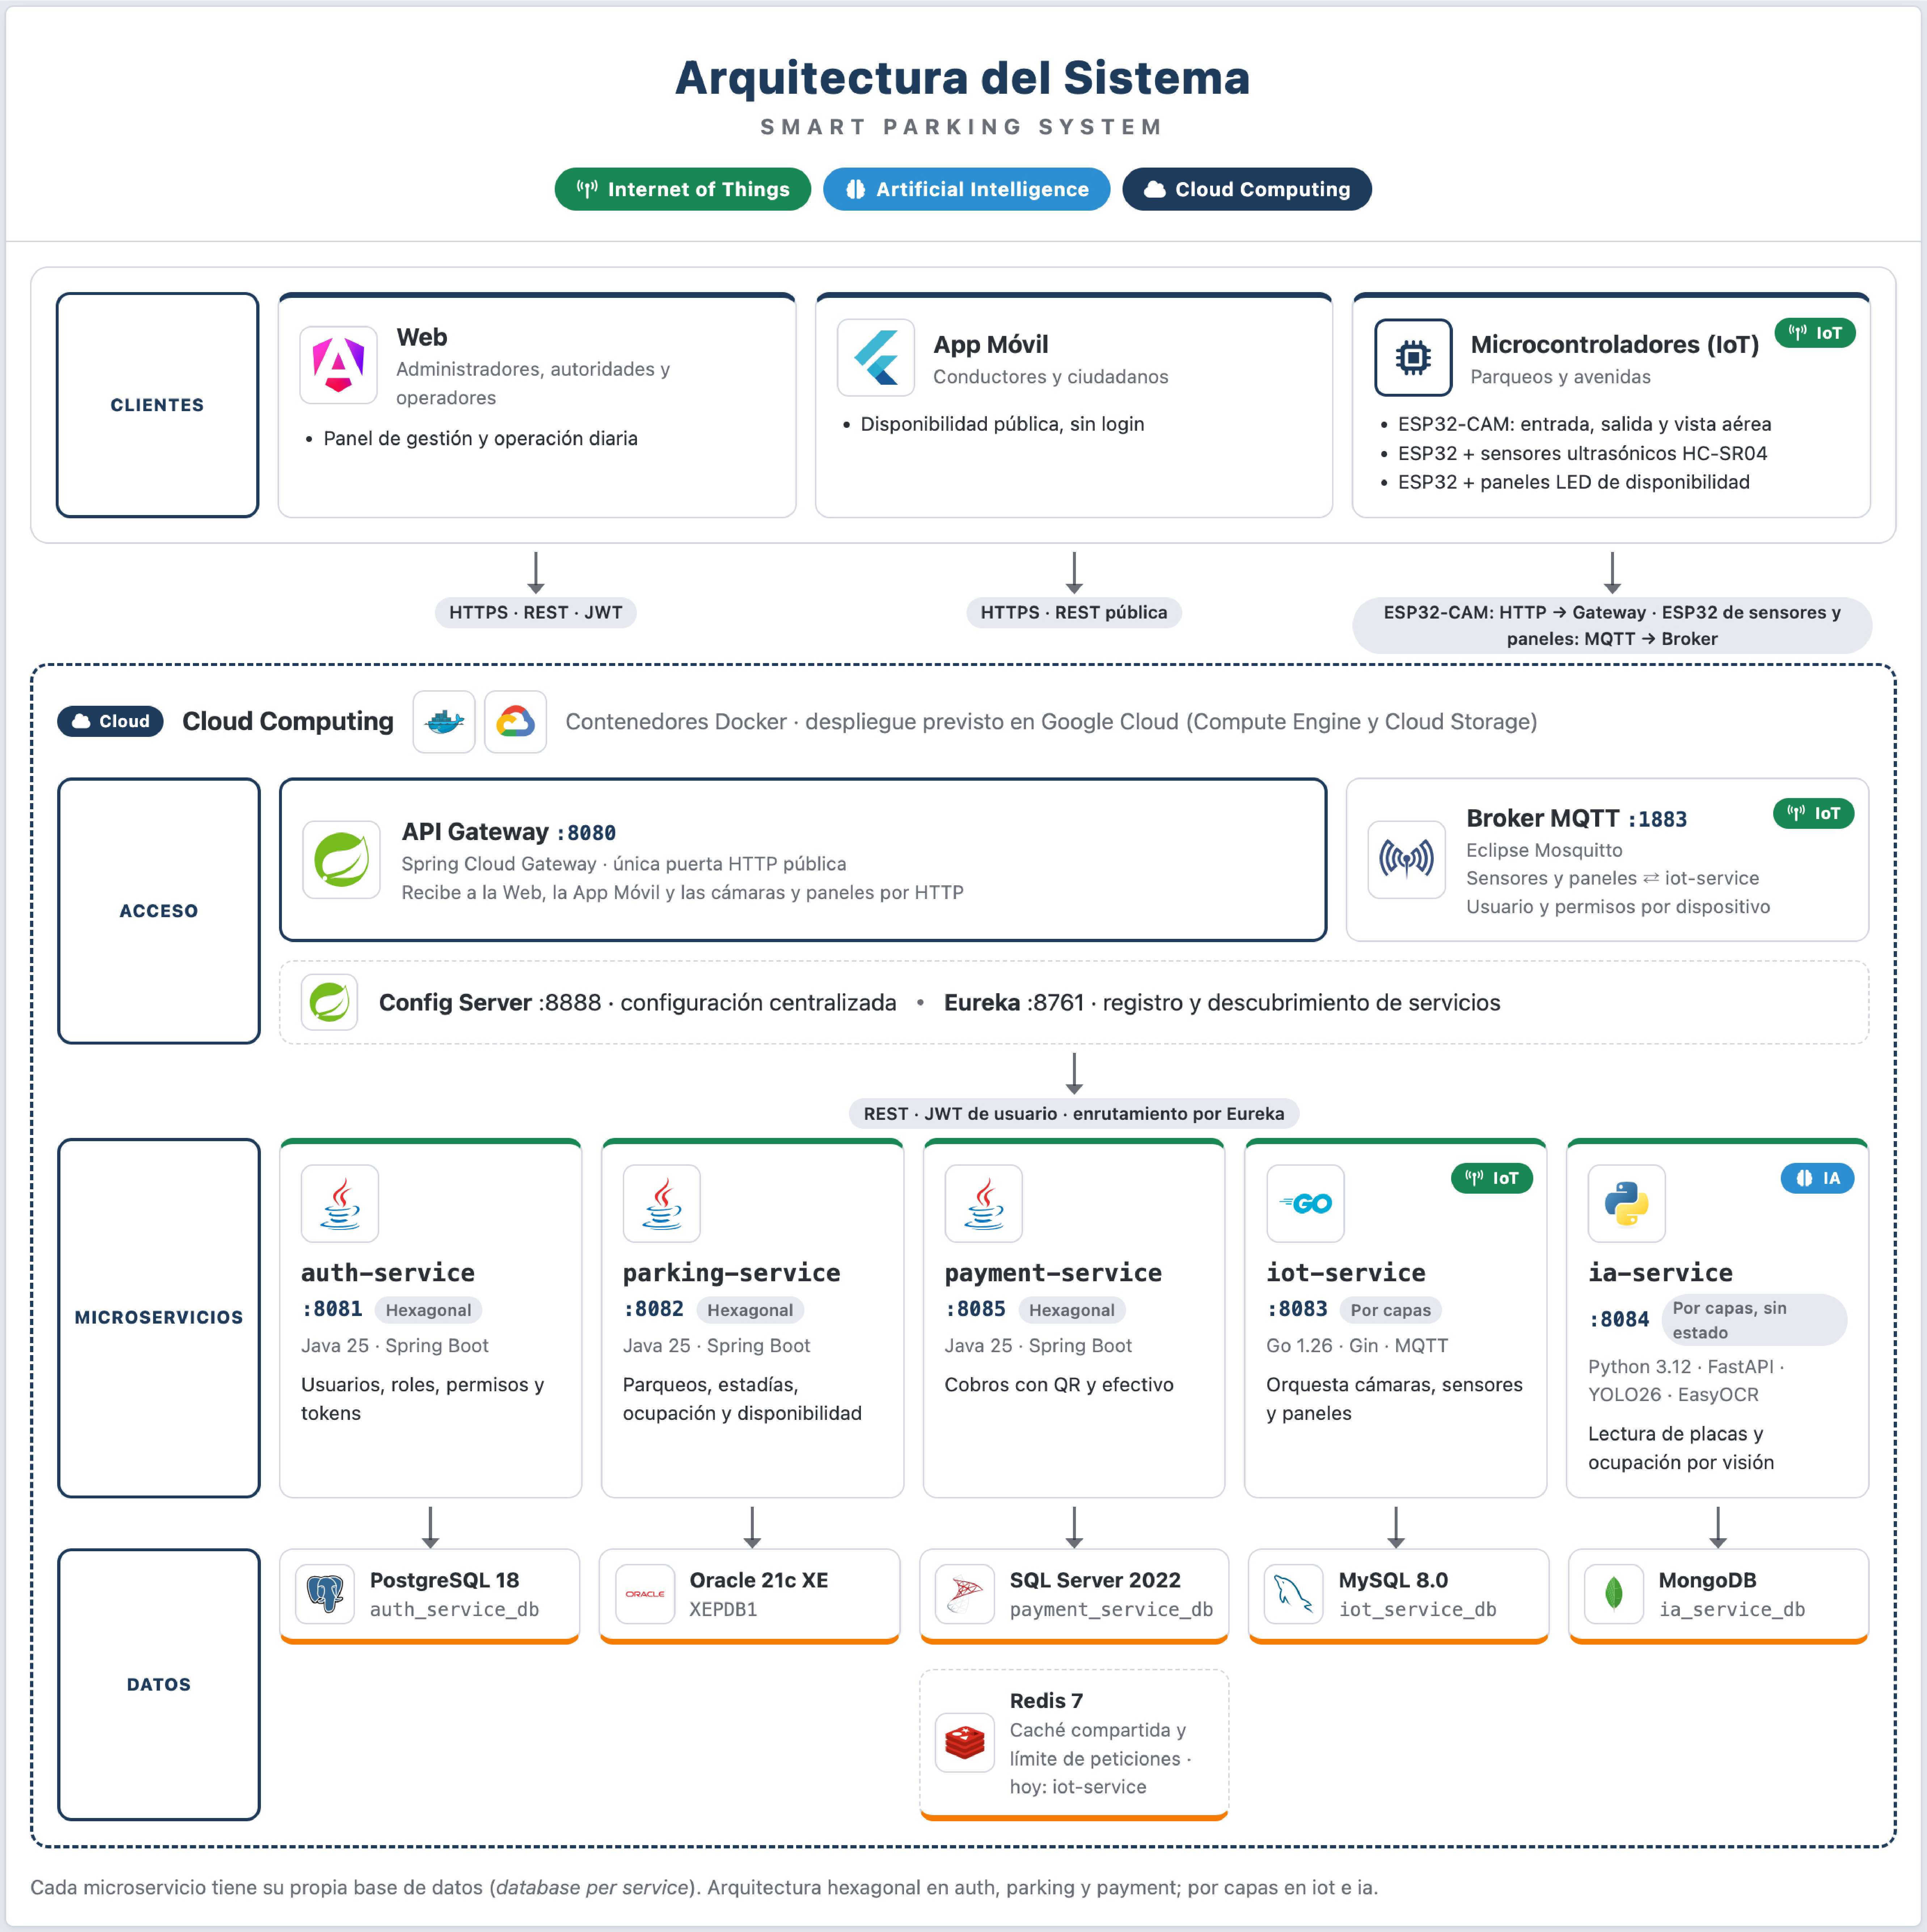
\includegraphics[width=1\textwidth]{anexos/arquitectura_sistema.pdf}
	
	\begin{flushleft}
		\setlength{\parskip}{0pt}
		\small \textit{Nota.} Arquitectura de sistema. \\ Fuente: Elaboración propia.
	\end{flushleft}
\end{figure}

% =========================================================================
% ANEXO 4: SOLICITUD DE AUTORIZACIÓN A LA MUNICIPALIDAD PROVINCIAL DE HUARAZ
% =========================================================================
\clearpage
\subsection{Anexo 4: Solicitud de autorización a la Municipalidad Provincial de Huaraz}

\noindent A continuación, se presenta la solicitud de autorización para realizar el estudio de tesis, presentada a la Municipalidad Provincial de Huaraz.

\vspace{-0.2cm}
\begin{figure}[H]
	\centering
	\captionsetup{format=plain, labelformat=simple, labelsep=newline, labelfont=bf, textfont=it, singlelinecheck=off}
	\caption{Solicitud de autorización presentada a la Municipalidad Provincial de Huaraz}
	\label{fig:anexo-solicitud-mph}
	\vspace{0.15cm}
	
	\fbox{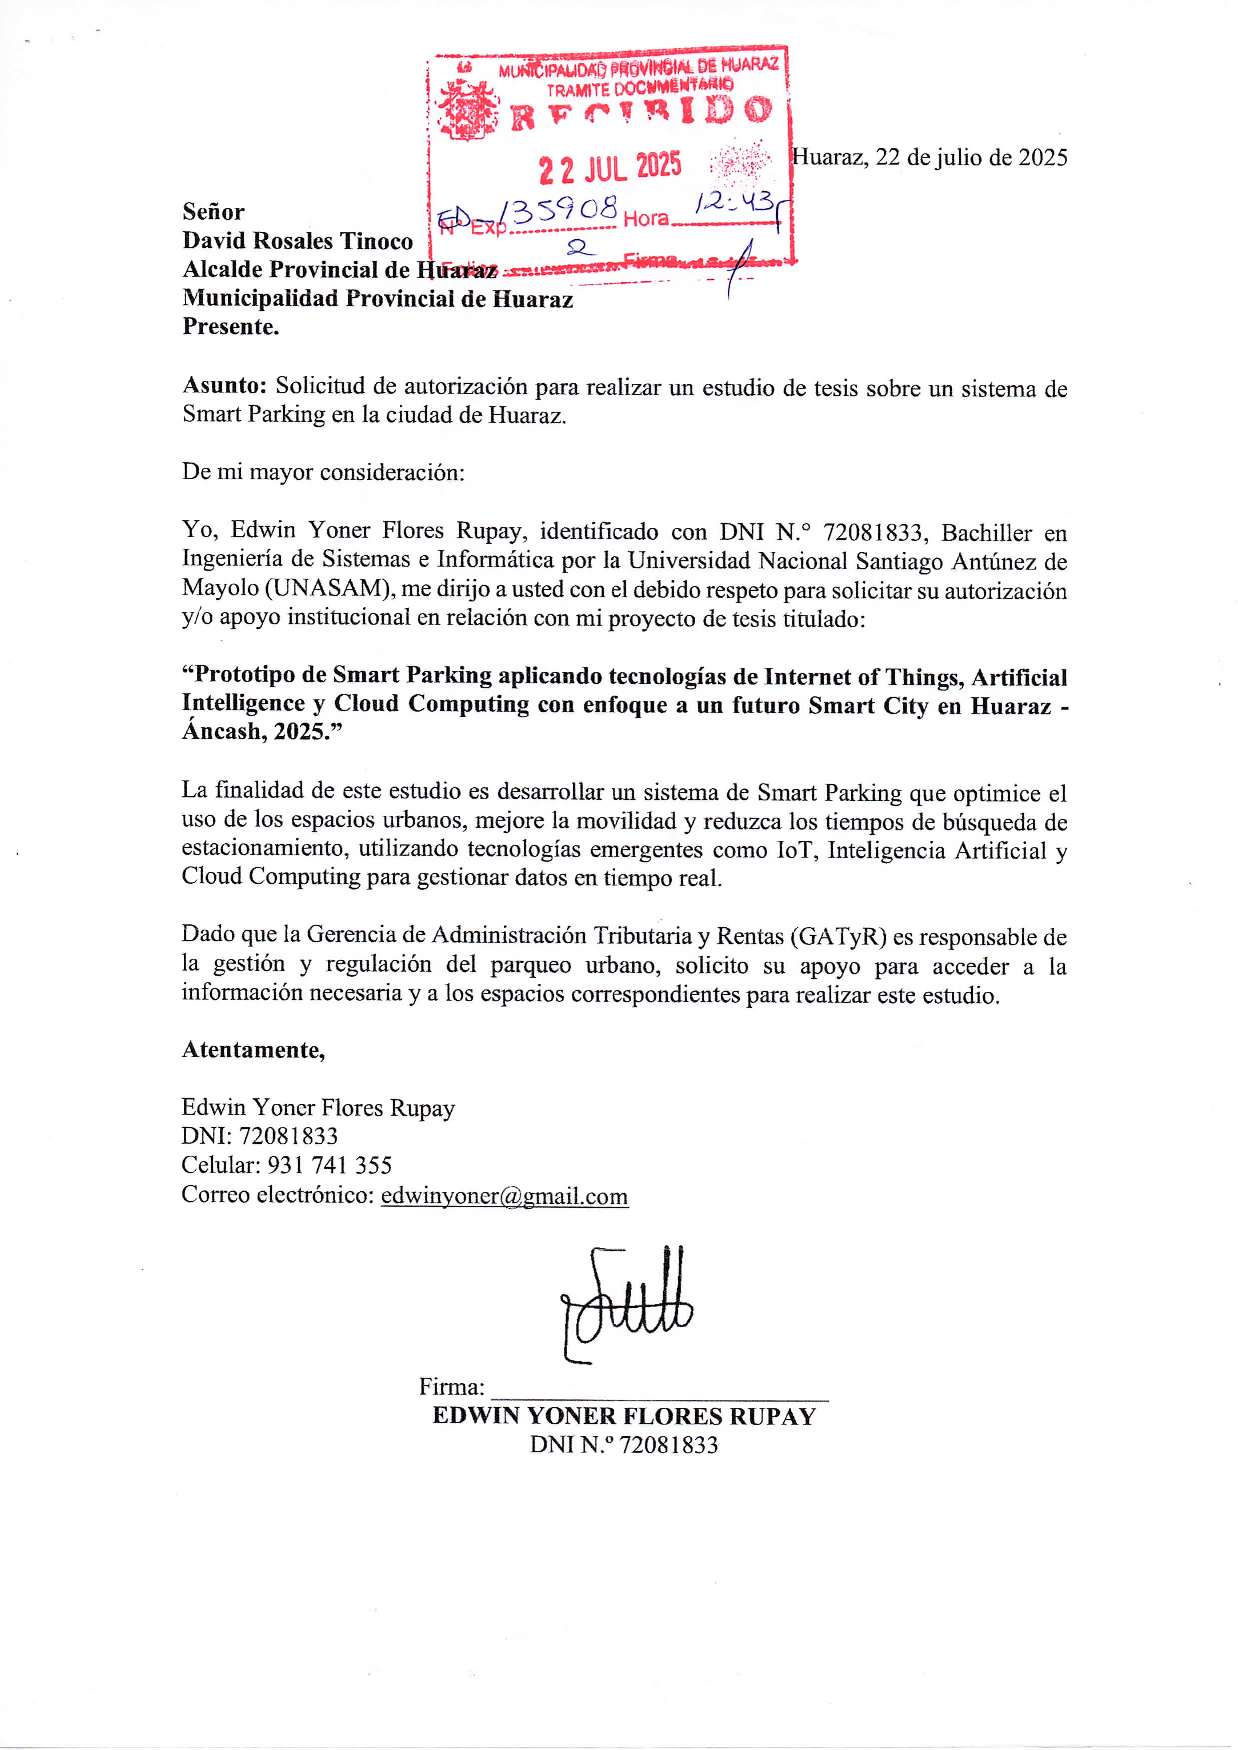
\includegraphics[height=0.66\textheight, width=0.95\textwidth, keepaspectratio]{anexos/solicitud.pdf}}
	
	\begin{flushleft}
		\setlength{\parskip}{0pt}
		\small \textit{Nota.} Solicitud recibida por trámite documentario el 22 de julio de 2025 (Expediente ED 135908). \\ Fuente: Elaboración propia.
	\end{flushleft}
\end{figure}

% =========================================================================
% ANEXO 5: CARTA DE AUTORIZACIÓN DE LA MUNICIPALIDAD PROVINCIAL DE HUARAZ
% =========================================================================
\clearpage
\subsection{Anexo 5: Carta de autorización de la Municipalidad Provincial de Huaraz}

\noindent A continuación, se presenta la carta con la que la Municipalidad Provincial de Huaraz autorizó la realización del trabajo de investigación.

\vspace{-0.2cm}
\begin{figure}[H]
	\centering
	\captionsetup{format=plain, labelformat=simple, labelsep=newline, labelfont=bf, textfont=it, singlelinecheck=off}
	\caption{Carta de autorización para realizar el trabajo de investigación}
	\label{fig:anexo-autorizacion-mph}
	\vspace{0.15cm}
	
	\fbox{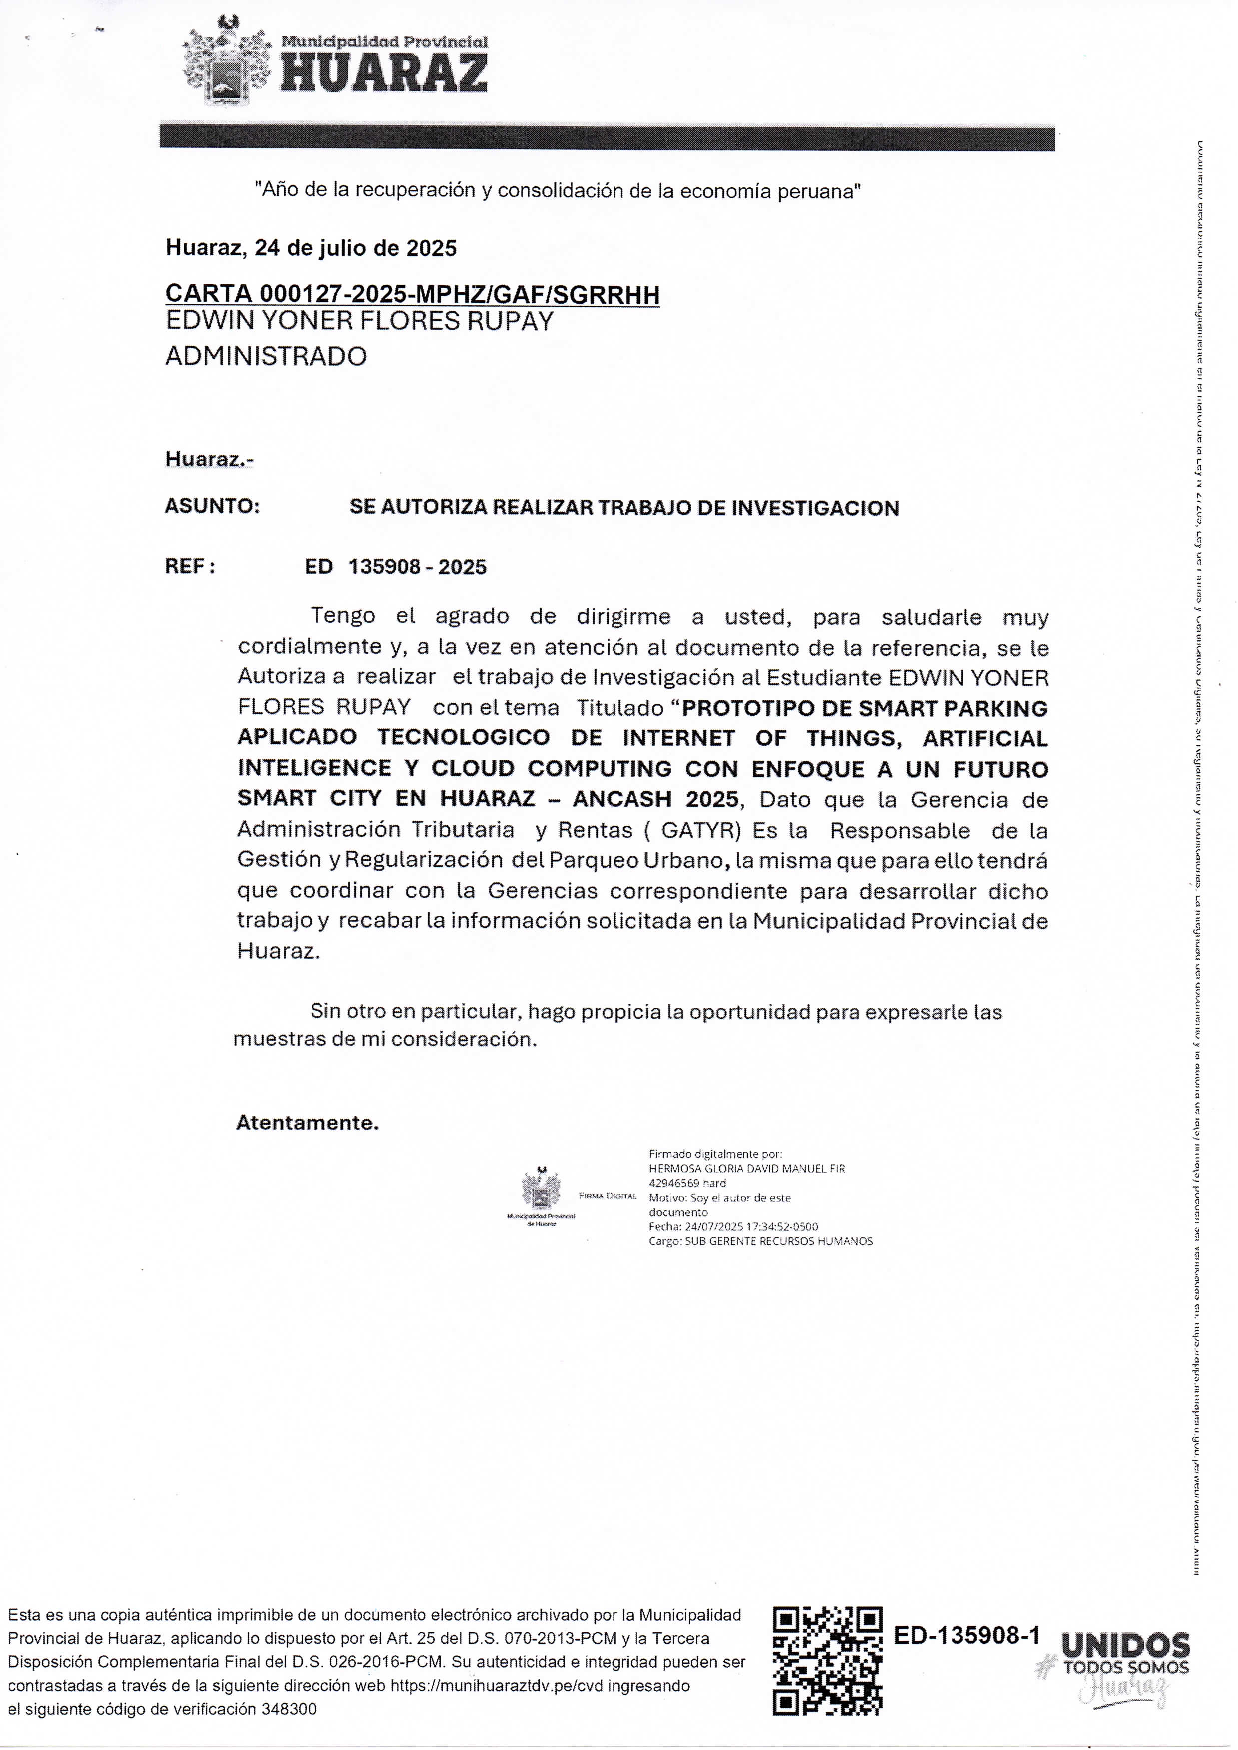
\includegraphics[height=0.66\textheight, width=0.95\textwidth, keepaspectratio]{anexos/autorización.pdf}}
	
	\begin{flushleft}
		\setlength{\parskip}{0pt}
		\small \textit{Nota.} Carta N.° 000127-2025-MPHZ/GAF/SGRRHH, del 24 de julio de 2025, con firma digital. \\ Fuente: Municipalidad Provincial de Huaraz (2025).
	\end{flushleft}
\end{figure}

\end{document}
